% Options for packages loaded elsewhere
\PassOptionsToPackage{unicode}{hyperref}
\PassOptionsToPackage{hyphens}{url}
\PassOptionsToPackage{dvipsnames,svgnames,x11names}{xcolor}
%
\documentclass[
  letterpaper,
  DIV=11,
  numbers=noendperiod]{scrreprt}

\usepackage{amsmath,amssymb}
\usepackage{iftex}
\ifPDFTeX
  \usepackage[T1]{fontenc}
  \usepackage[utf8]{inputenc}
  \usepackage{textcomp} % provide euro and other symbols
\else % if luatex or xetex
  \usepackage{unicode-math}
  \defaultfontfeatures{Scale=MatchLowercase}
  \defaultfontfeatures[\rmfamily]{Ligatures=TeX,Scale=1}
\fi
\usepackage{lmodern}
\ifPDFTeX\else  
    % xetex/luatex font selection
  \setmainfont[]{Calibri}
\fi
% Use upquote if available, for straight quotes in verbatim environments
\IfFileExists{upquote.sty}{\usepackage{upquote}}{}
\IfFileExists{microtype.sty}{% use microtype if available
  \usepackage[]{microtype}
  \UseMicrotypeSet[protrusion]{basicmath} % disable protrusion for tt fonts
}{}
\makeatletter
\@ifundefined{KOMAClassName}{% if non-KOMA class
  \IfFileExists{parskip.sty}{%
    \usepackage{parskip}
  }{% else
    \setlength{\parindent}{0pt}
    \setlength{\parskip}{6pt plus 2pt minus 1pt}}
}{% if KOMA class
  \KOMAoptions{parskip=half}}
\makeatother
\usepackage{xcolor}
\usepackage[a4paper,top=2cm,bottom=1cm,left=2.5cm,right=2.2cm,footskip=0.7cm]{geometry}
\ifLuaTeX
  \usepackage{luacolor}
  \usepackage[soul]{lua-ul}
\else
  \usepackage{soul}
  
\fi
\setlength{\emergencystretch}{3em} % prevent overfull lines
\setcounter{secnumdepth}{5}
% Make \paragraph and \subparagraph free-standing
\ifx\paragraph\undefined\else
  \let\oldparagraph\paragraph
  \renewcommand{\paragraph}[1]{\oldparagraph{#1}\mbox{}}
\fi
\ifx\subparagraph\undefined\else
  \let\oldsubparagraph\subparagraph
  \renewcommand{\subparagraph}[1]{\oldsubparagraph{#1}\mbox{}}
\fi


\providecommand{\tightlist}{%
  \setlength{\itemsep}{0pt}\setlength{\parskip}{0pt}}\usepackage{longtable,booktabs,array}
\usepackage{calc} % for calculating minipage widths
% Correct order of tables after \paragraph or \subparagraph
\usepackage{etoolbox}
\makeatletter
\patchcmd\longtable{\par}{\if@noskipsec\mbox{}\fi\par}{}{}
\makeatother
% Allow footnotes in longtable head/foot
\IfFileExists{footnotehyper.sty}{\usepackage{footnotehyper}}{\usepackage{footnote}}
\makesavenoteenv{longtable}
\usepackage{graphicx}
\makeatletter
\def\maxwidth{\ifdim\Gin@nat@width>\linewidth\linewidth\else\Gin@nat@width\fi}
\def\maxheight{\ifdim\Gin@nat@height>\textheight\textheight\else\Gin@nat@height\fi}
\makeatother
% Scale images if necessary, so that they will not overflow the page
% margins by default, and it is still possible to overwrite the defaults
% using explicit options in \includegraphics[width, height, ...]{}
\setkeys{Gin}{width=\maxwidth,height=\maxheight,keepaspectratio}
% Set default figure placement to htbp
\makeatletter
\def\fps@figure{htbp}
\makeatother

\usepackage{booktabs}
\usepackage{caption}
\usepackage{longtable}
\usepackage{colortbl}
\usepackage{array}
% \usepackage{libertine} % so we can see the checkmarks in the intro
\usepackage{xcolor}
\usepackage{ragged2e} % for justifying text in multiple column layout

\RedeclareSectionCommand[
  beforeskip=0pt,
  afterskip=2pt]{chapter} %so to remove the word chapter and the space before

\setsansfont{Calibri}

\definecolor{MyBlue}{RGB}{54,95,145}
\addtokomafont{chapter}{\color{MyBlue}}
\addtokomafont{chapterprefix}{\color{MyBlue}}
\addtokomafont{chapter}{\fontsize{14pt}{14pt}\selectfont}
\addtokomafont{chapterprefix}{\fontsize{14pt}{14pt}\selectfont}

\addtokomafont{section}{\color{MyBlue}}
\addtokomafont{section}{\fontsize{12pt}{12pt}\selectfont}

\newenvironment{tightcenter}{%
  \setlength\topsep{5pt}
  \setlength\parskip{0pt}
  \bfseries
  \begin{center}
}{%
  \end{center}
}
\KOMAoption{captions}{tableheading}
\makeatletter
\@ifpackageloaded{tcolorbox}{}{\usepackage[skins,breakable]{tcolorbox}}
\@ifpackageloaded{fontawesome5}{}{\usepackage{fontawesome5}}
\definecolor{quarto-callout-color}{HTML}{909090}
\definecolor{quarto-callout-note-color}{HTML}{0758E5}
\definecolor{quarto-callout-important-color}{HTML}{CC1914}
\definecolor{quarto-callout-warning-color}{HTML}{EB9113}
\definecolor{quarto-callout-tip-color}{HTML}{00A047}
\definecolor{quarto-callout-caution-color}{HTML}{FC5300}
\definecolor{quarto-callout-color-frame}{HTML}{acacac}
\definecolor{quarto-callout-note-color-frame}{HTML}{4582ec}
\definecolor{quarto-callout-important-color-frame}{HTML}{d9534f}
\definecolor{quarto-callout-warning-color-frame}{HTML}{f0ad4e}
\definecolor{quarto-callout-tip-color-frame}{HTML}{02b875}
\definecolor{quarto-callout-caution-color-frame}{HTML}{fd7e14}
\makeatother
\makeatletter
\@ifpackageloaded{bookmark}{}{\usepackage{bookmark}}
\makeatother
\makeatletter
\@ifpackageloaded{caption}{}{\usepackage{caption}}
\AtBeginDocument{%
\ifdefined\contentsname
  \renewcommand*\contentsname{Table of contents}
\else
  \newcommand\contentsname{Table of contents}
\fi
\ifdefined\listfigurename
  \renewcommand*\listfigurename{List of Figures}
\else
  \newcommand\listfigurename{List of Figures}
\fi
\ifdefined\listtablename
  \renewcommand*\listtablename{List of Tables}
\else
  \newcommand\listtablename{List of Tables}
\fi
\ifdefined\figurename
  \renewcommand*\figurename{Figure}
\else
  \newcommand\figurename{Figure}
\fi
\ifdefined\tablename
  \renewcommand*\tablename{Table}
\else
  \newcommand\tablename{Table}
\fi
}
\@ifpackageloaded{float}{}{\usepackage{float}}
\floatstyle{ruled}
\@ifundefined{c@chapter}{\newfloat{codelisting}{h}{lop}}{\newfloat{codelisting}{h}{lop}[chapter]}
\floatname{codelisting}{Listing}
\newcommand*\listoflistings{\listof{codelisting}{List of Listings}}
\makeatother
\makeatletter
\makeatother
\makeatletter
\@ifpackageloaded{caption}{}{\usepackage{caption}}
\@ifpackageloaded{subcaption}{}{\usepackage{subcaption}}
\makeatother
\ifLuaTeX
  \usepackage{selnolig}  % disable illegal ligatures
\fi
\usepackage{bookmark}

\IfFileExists{xurl.sty}{\usepackage{xurl}}{} % add URL line breaks if available
\urlstyle{same} % disable monospaced font for URLs
\hypersetup{
  pdftitle={High-level Summary Report on Preliminary ACE 2022 Data},
  pdfauthor={Performance Review Unit},
  colorlinks=true,
  linkcolor={blue},
  filecolor={Maroon},
  citecolor={Blue},
  urlcolor={Blue},
  pdfcreator={LaTeX via pandoc}}

\title{High-level Summary Report on Preliminary ACE 2022 Data}
\author{Performance Review Unit}
\date{2023-12-15}

\begin{document}
\maketitle

\renewcommand*\contentsname{Table of contents}
{
\hypersetup{linkcolor=}
\setcounter{tocdepth}{2}
\tableofcontents
}
\listoffigures
\bookmarksetup{startatroot}

\chapter*{Welcome}\label{welcome}
\addcontentsline{toc}{chapter}{Welcome}

\markboth{Welcome}{Welcome}

This document provides a first insight on the level of 2022
cost-effectiveness performance both for the Pan-European system and for
individual ANSPs before the official release of the next ACE
benchmarking report.

This document is available for download as a
\href{https://www.eurocontrol.int/sites/default/files/2023-12/eurocontrol-summary-report-preliminary-ace-2022-data.pdf}{PDF
version}.

\subsection*{IMPORTANT NOTICE}\label{important-notice}
\addcontentsline{toc}{subsection}{IMPORTANT NOTICE}

{Data contained in this document are preliminary and subject to changes
before the publication of the final ACE benchmarking report in May
2024.}

\bookmarksetup{startatroot}

\chapter{Introduction}\label{dec-intro}

The ACE benchmarking work is commissioned by the Performance Review
Commission (PRC) and carried out by the EUROCONTROL Performance Review
Unit (PRU) using information provided by Air Navigation Services
Providers (ANSPs) in compliance with Decision No.~88 of the Permanent
Commission of EUROCONTROL on economic information disclosure\footnote{Due
  to the on-going war in Ukraine, UkSATSE has been excluded from the ACE
  analysis.}.

The data processing, analysis and reporting are conducted with the
assistance of the ACE Working Group, which comprises representatives
from participating ANSPs, airspace users, regulatory authorities and the
Performance Review Unit. This enables participants to share experiences
and establish a common understanding of underlying assumptions and data
limitations.

The objective of this document is to provide a first insight on the
level of 2022 cost-effectiveness performance both for the Pan-European
system and for individual ANSPs before the release of the final ACE
benchmarking report, which is planned end of May 2024. Economic
information disclosure by ANSPs takes time as it is depending on the
publication of their audited financial statements, which can be a
lengthy process. This document also presents specific financial
indicators, extracted from the
\href{https://ansperformance.eu/economics/finance/}{ANSPs Financial
Indicators Dashboard}, that can be used to monitor potential cash and
liquidity issues experienced by ANSPs as a result of the COVID-19
pandemic.

The final ACE benchmarking report will provide more detailed information
on observed changes for selected performance indicators both at
pan-European system level and at ANSP level. This detailed analysis will
particularly focus on ANSPs for which significant differences in costs
are observed. The report will present the main drivers underlying these
differences.

In addition, a new theme will be developed, examining the potential
impact of different regulatory, institutional, and corporate governance
setups on ANSPs economic performance. While acknowledging that there are
many different factors influencing the conduct of organisations (see the
ACE Handbook for a comprehensive overview of endogenous and exogenous
\href{https://ansperformance.eu/economics/ace/ace-handbook/influencing-factors.html}{factors
affecting performance}), the forthcoming ACE report will provide new
analysis considering differences in the legal status, ownership, and
decision-making arrangements among ANSPs.

Figure~\ref{fig-figure-1-1} illustrates the timeline to produce the next
ACE benchmarking report.

\begin{figure}

\centering{

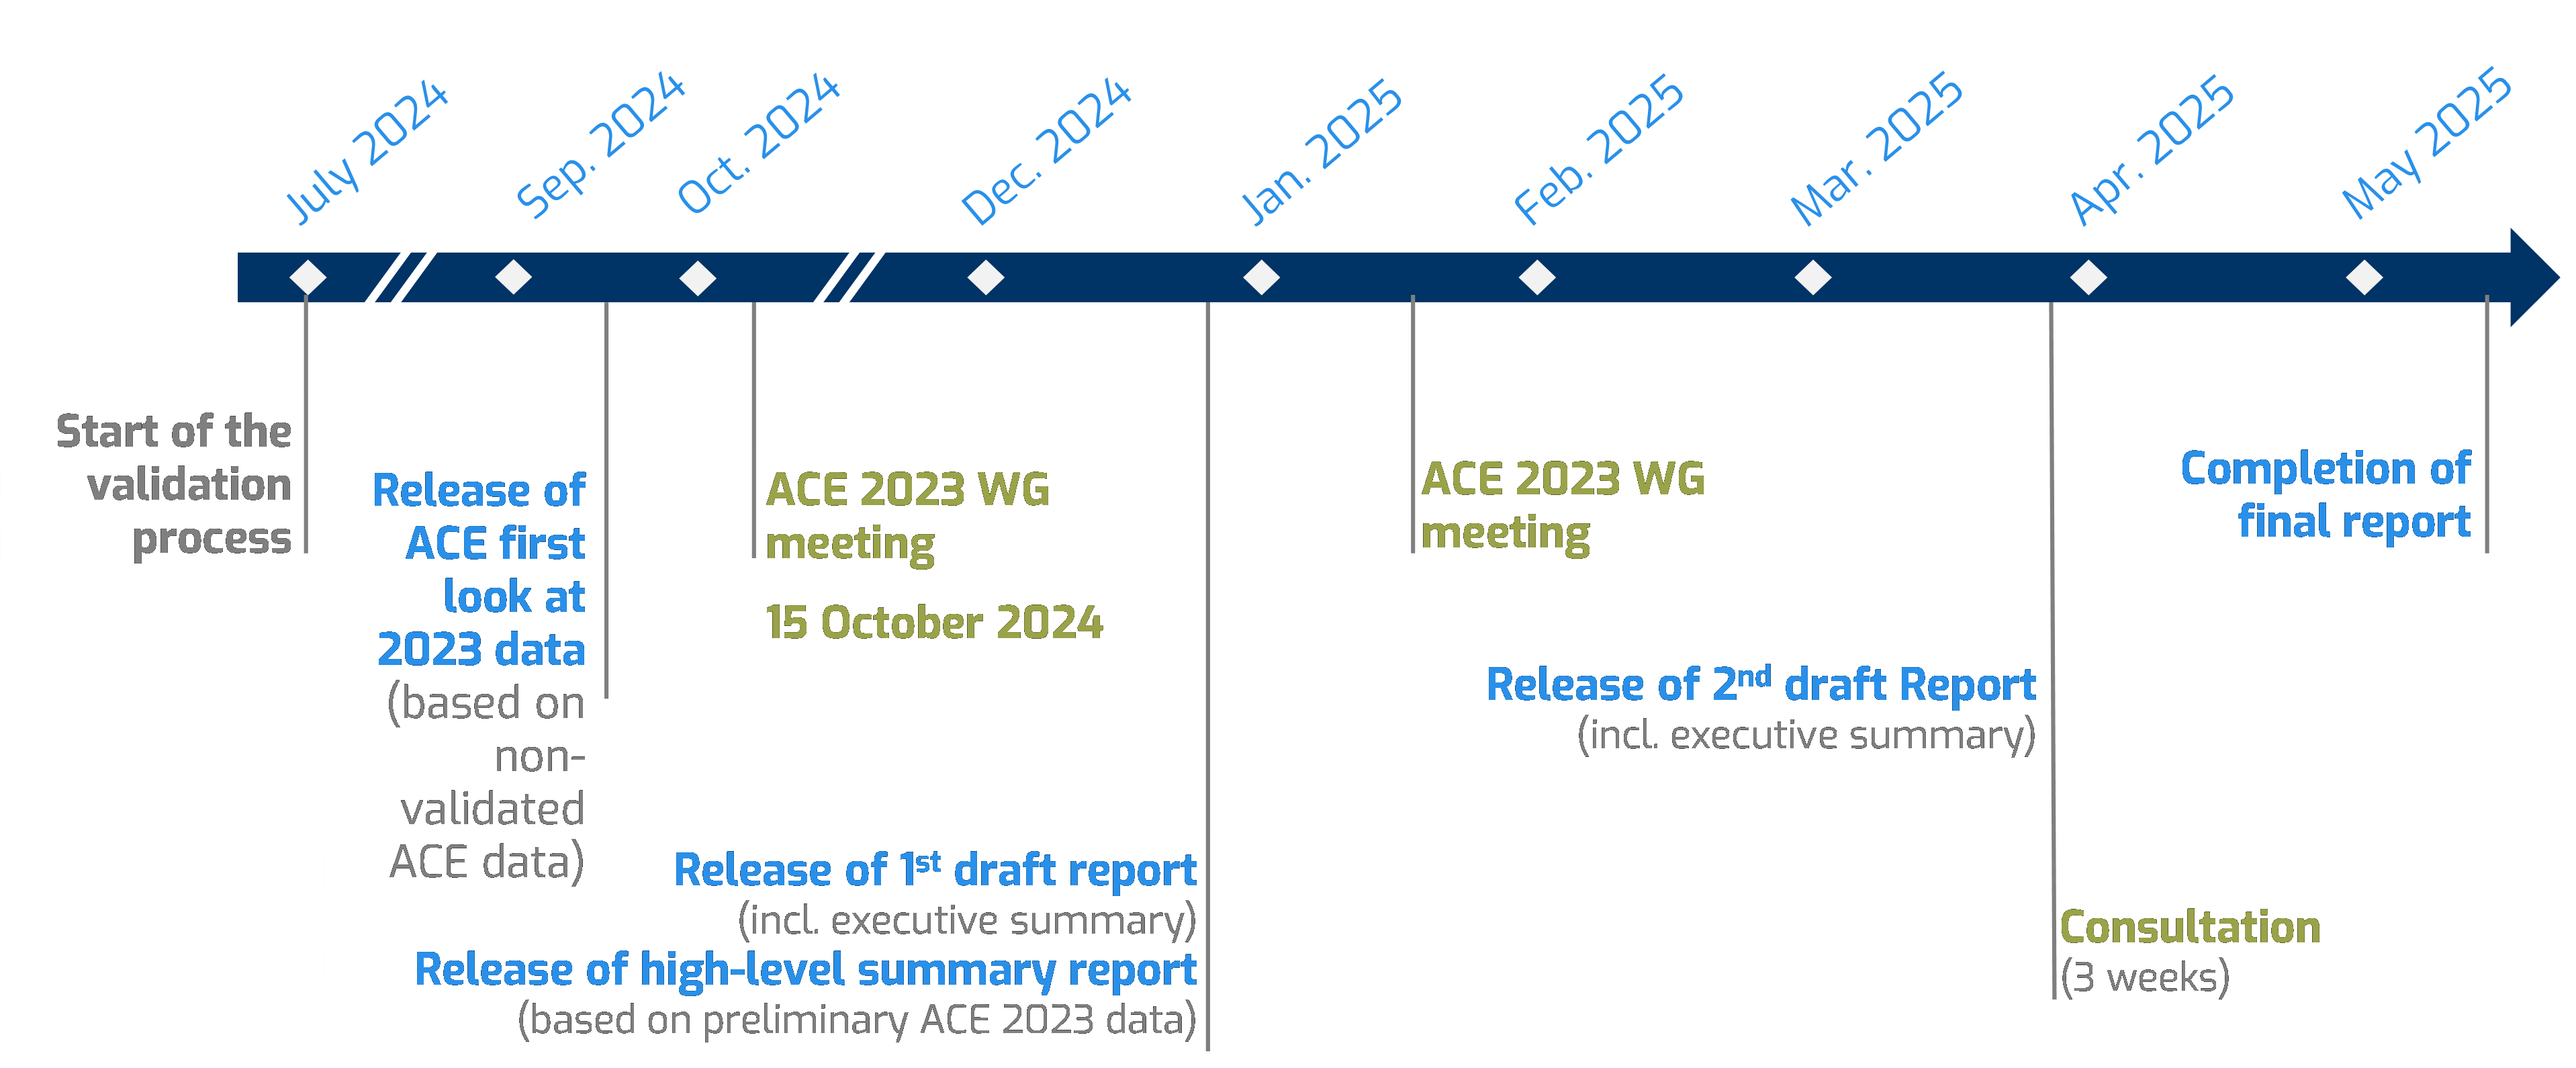
\includegraphics[width=1\textwidth,height=\textheight]{figures/figure1-1_transp.png}

}

\caption{\label{fig-figure-1-1}Timeline to produce the next ACE
benchmarking report}

\end{figure}%

It is important that robust ACE benchmarking analysis is available in a
timely manner since several stakeholders, most notably ANSPs'
management, regulatory authorities (e.g.~NSAs) and airspace users, have
a keen interest in receiving the information in the ACE reports as early
as possible.

Seventeen out of 38 ANSPs submitted their ACE 2022 data on time by the
1st of July 2023 and, all data submissions were received by the end of
August 2023. Overall, this constitutes a major improvement compared to
previous years. Clearly, the timescale to produce the ACE benchmarking
report is inevitably delayed if data are not submitted on time.

It should be noted that the data presented in this document are still
\ul{preliminary and not yet fully validated}. Indeed, the data
submission milestone is just the first step of a process which comprises
a thorough verification and analysis of individual ANSP submissions.
This validation exercise also includes a formal round of exchange
between the PRU and each ANSP in order to ensure a common understanding
of the data submitted by the ANSP.

The data used in this document reflects the information stored in the
ACE database on the 5th December 2023. Figure~\ref{fig-figure-1-2} shows
the status of the ACE data validation process for the data presented in
this document.

\begin{figure}

\centering{

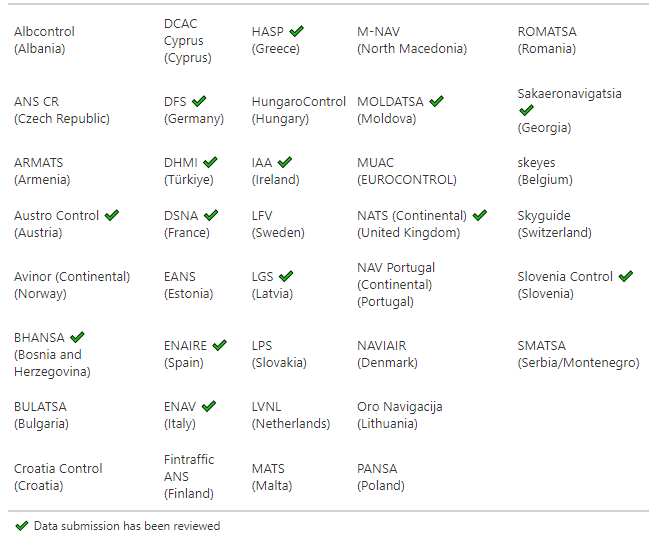
\includegraphics[width=0.9\textwidth,height=0.9\textheight]{figures/ansp_status_table.PNG}

}

\caption{\label{fig-figure-1-2}Status of 2022 data validation process}

\end{figure}%

The data contained in this report is therefore subject to changes before
the release of the final ACE 2022 benchmarking report in May 2024.

The remainder of this report is structured as follows:

\begin{itemize}
\tightlist
\item
  Chapter~\ref{sec-high}: provides a high-level presentation of 2022
  revenues, costs and staff data.
\item
  Chapter~\ref{sec-economic}: presents a preliminary analysis of
  economic cost-effectiveness at Pan-European and ANSP level.
\item
  Chapter~\ref{sec-financial}: presents a preliminary analysis of
  financial cost-effectiveness at Pan-European and ANSP level, and
  underlying components.
\item
  Chapter~\ref{sec-covid}: presents a preliminary analysis of specific
  financial indicators at Pan-European and ANSP level.
\end{itemize}

\bookmarksetup{startatroot}

\chapter{High-level revenues, costs and staff data}\label{sec-high}

This chapter provides a \ul{preliminary} overview of high-level
revenues, costs and staff data provided in ANSPs ACE 2022 data
submissions. Total ANS revenues in 2022 amounted to €9 024M. Most
en-route revenues come from the collection of en-route charges (95.9\%,
see left pie chart). The proportion of terminal revenues from charges is
lower (68.3\%, see right pie chart), as additional income may directly
come from airport operators (21.3\%) through, for example, a contractual
arrangement between the ANSP and the airport operator).

\begin{figure}

\centering{

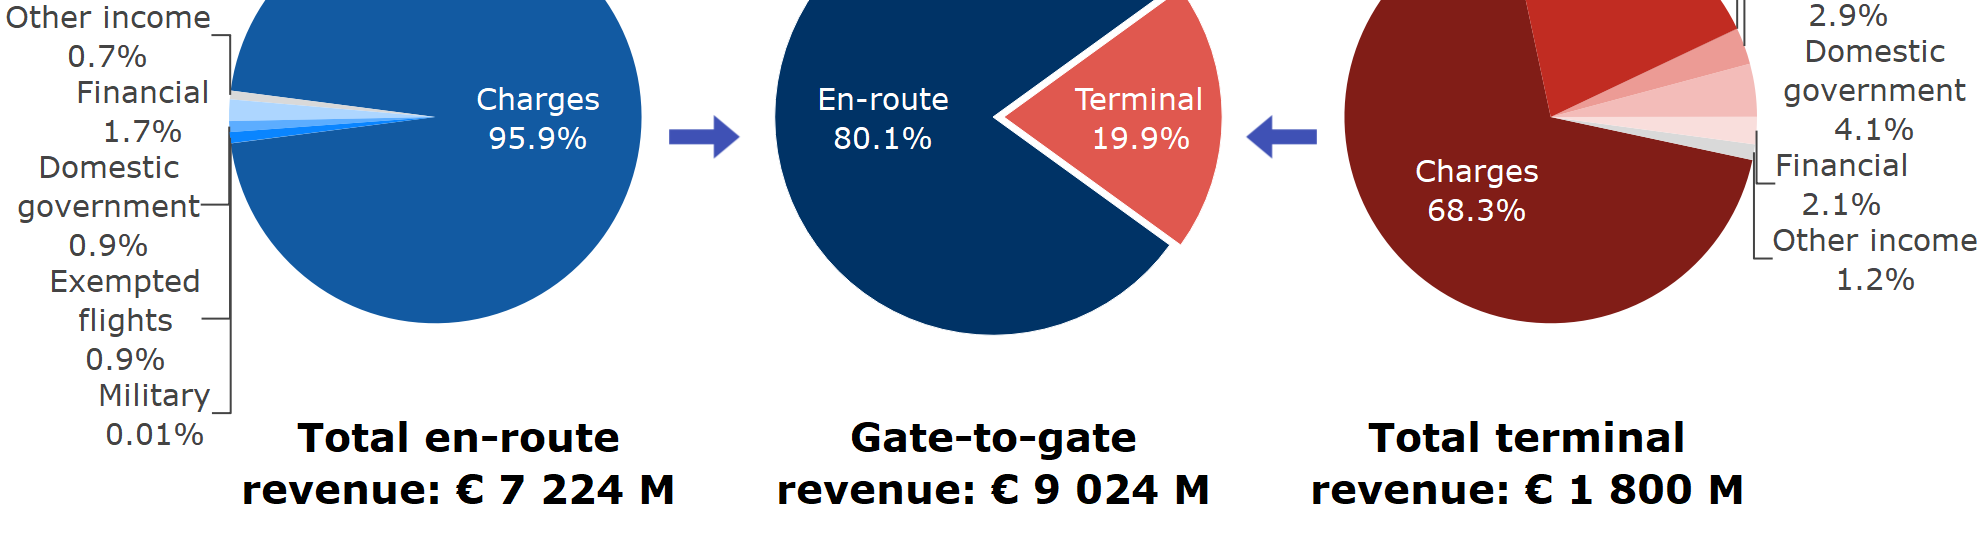
\includegraphics[width=1\textwidth,height=1\textheight]{figures/figure-2-1-hlsr_rev_pie.png}

\newlength\holdLTleft\newlength\holdLTright\setlength\holdLTleft{\LTleft}\relax\setlength\holdLTright{\LTright}\relax\setlength\LTleft{0\linewidth}

\setlength\LTright{0\linewidth}

\begin{longtable*}{@{\extracolsep{\fill}}rrcrr}
\toprule
En-route & \% & Gate-togate revenues (€ M) &  \% & Terminal \\ 
\midrule\addlinespace[2.5pt]
6 928 & 95.9\% & Income from charges & 68.3\% & 1 229 \\ 
n.a. & n.a. & Income from airport operators & 21.3\% &   383 \\ 
    1.0 & 0.01\% & Income from the military & 0.04\% &     0.7 \\ 
   63 & 0.9\% & Income in respect of exempted flights & 2.9\% &    51 \\ 
   62 & 0.9\% & Income from domestic goverment & 4.1\% &    75 \\ 
  122 & 1.7\% & Financial income & 2.1\% &    38 \\ 
   49 & 0.7\% & Other income (incl. exceptional revenue item) & 1.2\% &    22 \\ 
\cellcolor[HTML]{C0C0C0}{7 224} & \cellcolor[HTML]{C0C0C0}{100\%} & \cellcolor[HTML]{C0C0C0}{} & \cellcolor[HTML]{C0C0C0}{100\%} & \cellcolor[HTML]{C0C0C0}{1 800} \\ 
\bottomrule
\end{longtable*}
\setlength\LTleft{\holdLTleft}
\setlength\LTright{\holdLTright}

}

\caption{\label{fig-figure-2-1}Breakdown of gate-to-gate ANS revenues,
2022}

\end{figure}%

\begin{tcolorbox}[enhanced jigsaw, leftrule=.75mm, breakable, left=2mm, colframe=quarto-callout-note-color-frame, rightrule=.15mm, colback=white, opacityback=0, arc=.35mm, toprule=.15mm, bottomrule=.15mm]

\begin{figure}[H]

\begin{minipage}{0.30\linewidth}
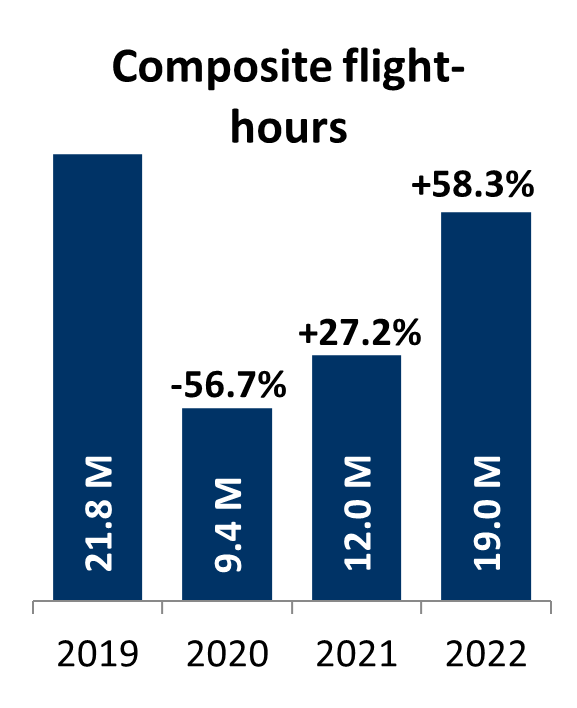
\includegraphics{figures/Figure-2-2-cfh.png}\end{minipage}%
%
\begin{minipage}{0.40\linewidth}

\justifying \noindent \hfill\break \hfill\break Across the Pan-European
system, traffic in 2022 (measured in composite flight-hours) was +58.3\%
higher than in 2021 but remained -13.3\% lower than in 2019. In the
meantime, total gate-to-gate revenues increased slightly less than
traffic (+55.3\%) and remained -14.9\% lower than in
2019.\end{minipage}%
%
\begin{minipage}{0.30\linewidth}
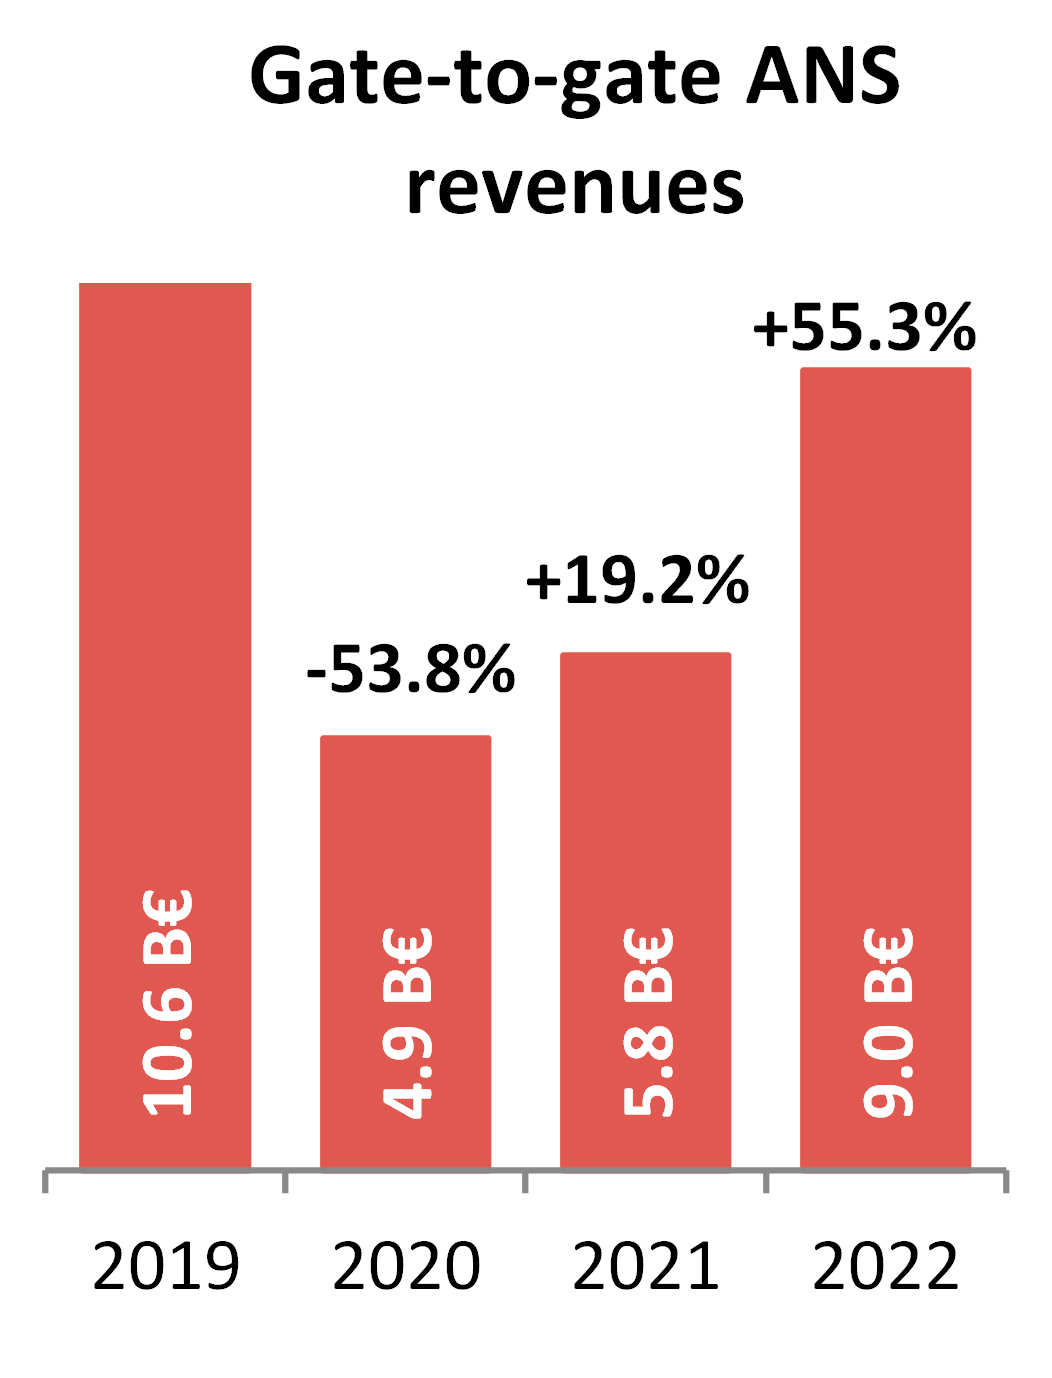
\includegraphics{figures/Figure-2-2-rev.png}\end{minipage}%

\end{figure}%

\end{tcolorbox}

\newpage{}

At ANSP level, a wide range of recovery rates is observed (from -51\% to
+14\%, see Figure~\ref{fig-Traffic_map}). The war in Ukraine also
resulted in airspace closures and reciprocal sanctions on air carriers
which impacted traffic flows in Europe. This inevitably impacts the
levels and trends of ACE indicators for the ANSPs being most affected by
the changes in traffic patterns.

\begin{figure}

\centering{

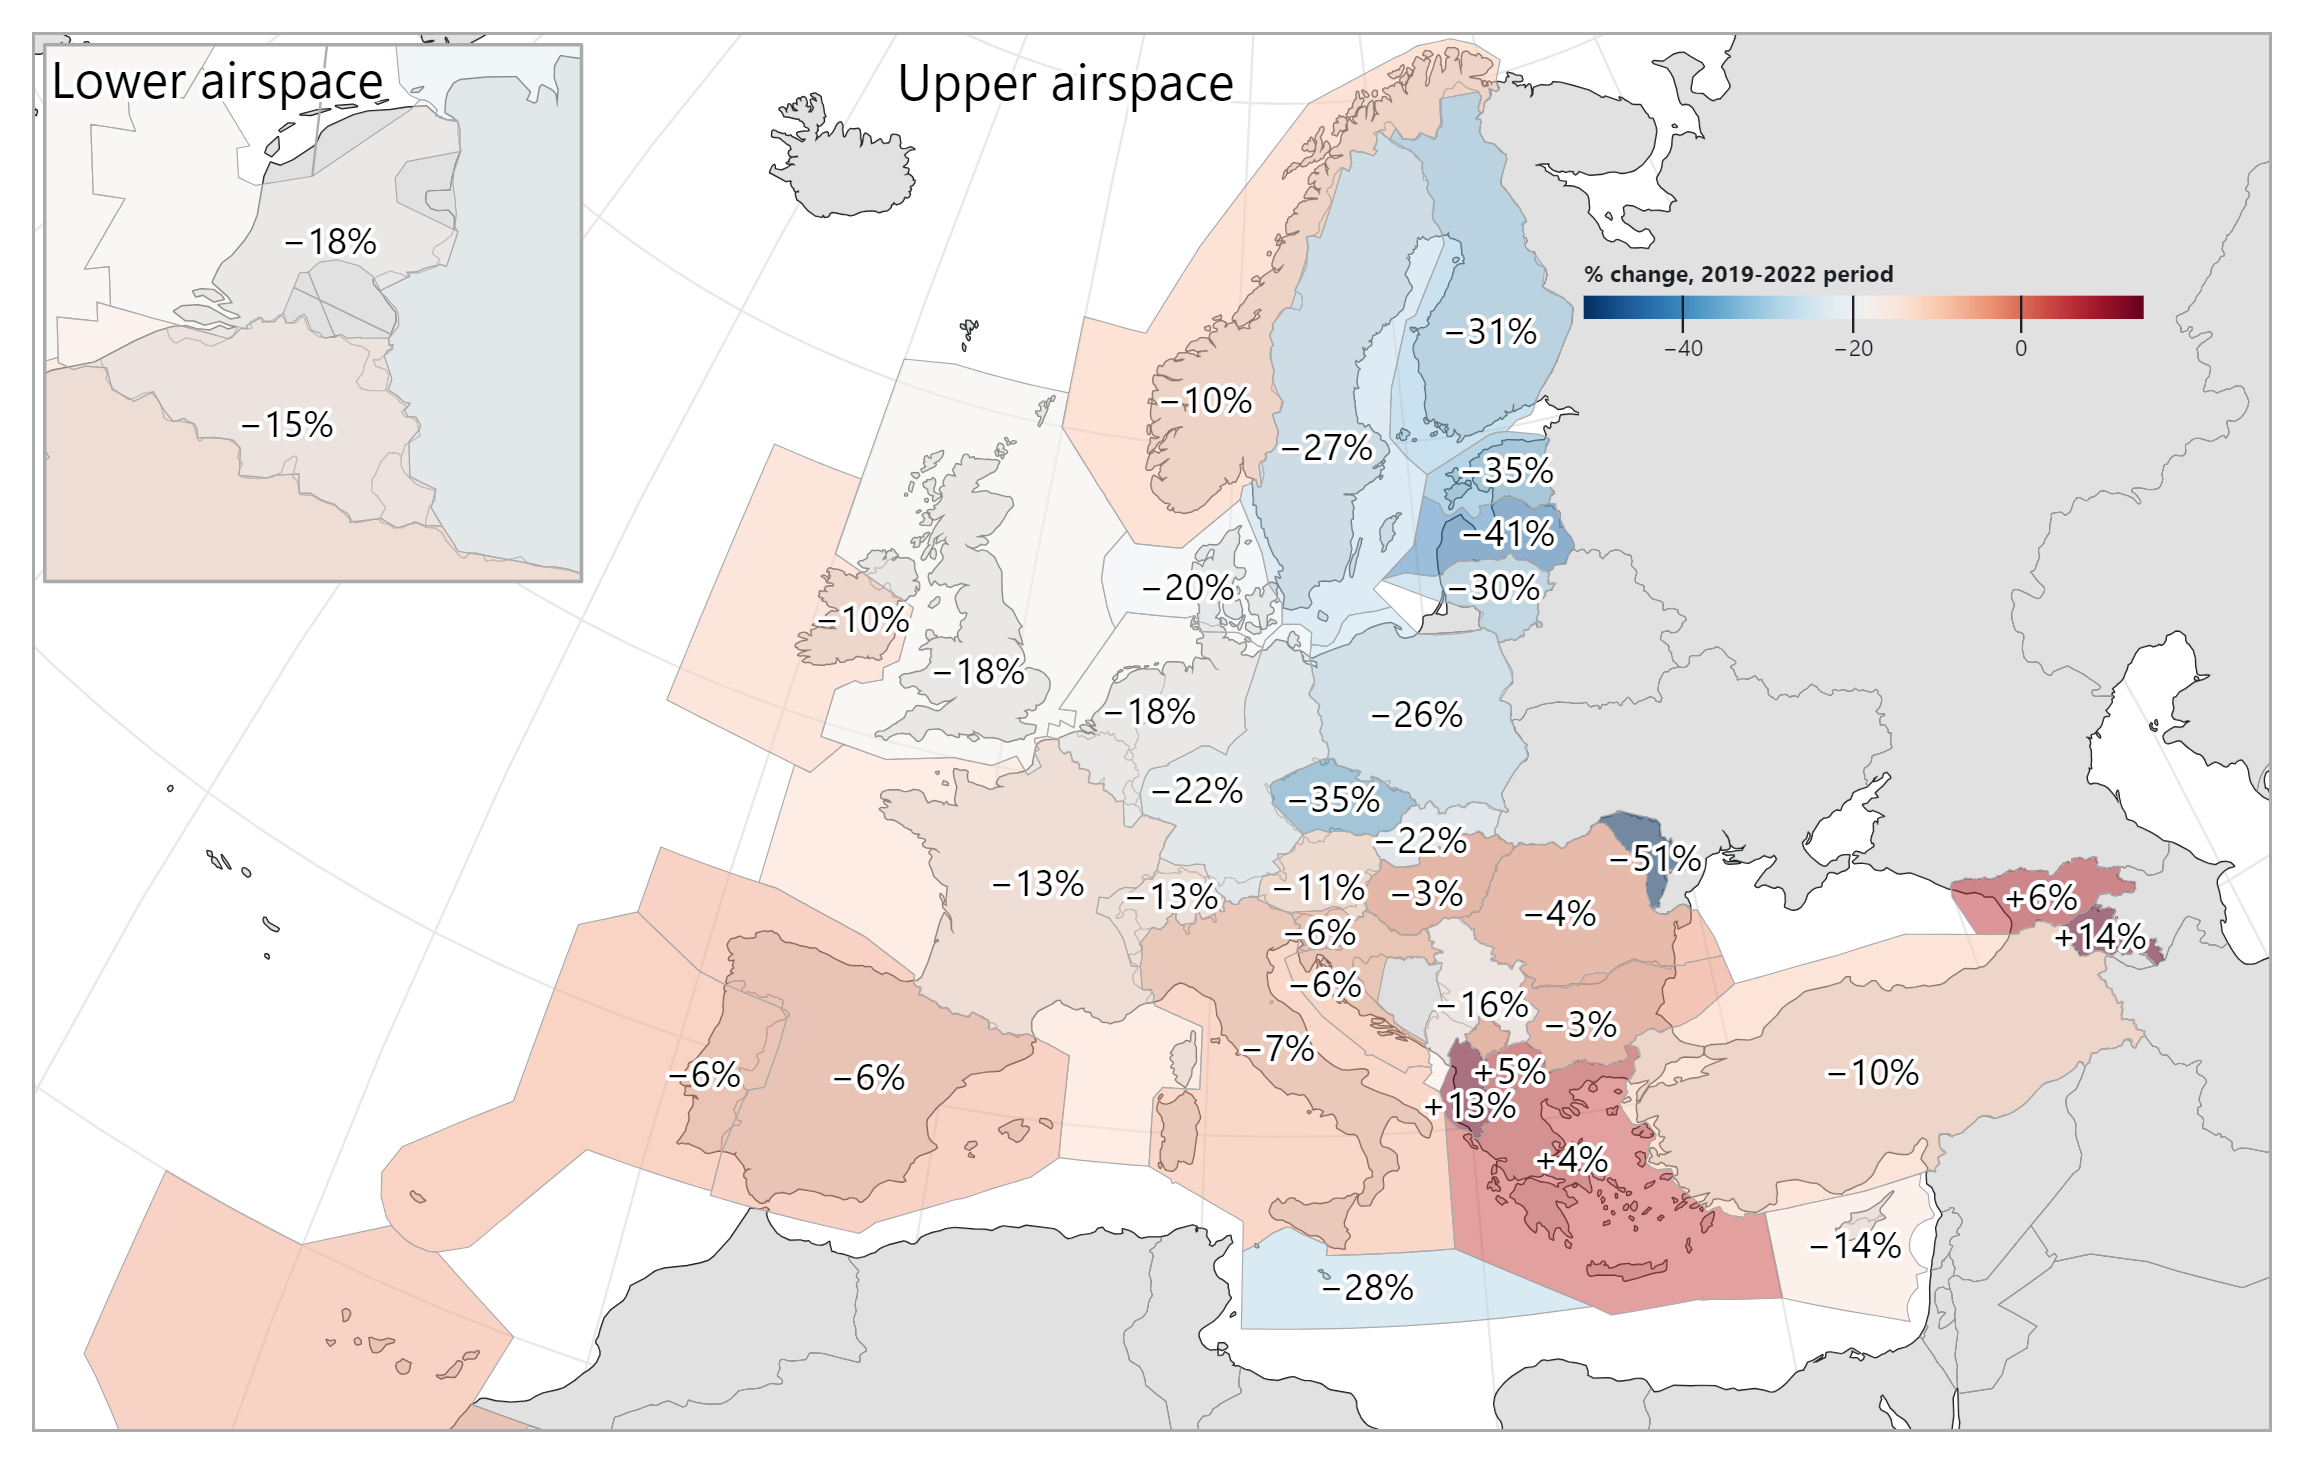
\includegraphics{figures/Traffic_map.png}

}

\caption{\label{fig-Traffic_map}Changes in composite flight-hours
between 2019 and 2022}

\end{figure}%

The ACE benchmarking analysis focuses on the specific costs of providing
gate-to-gate ATM/CNS services which amounted to €8 921M in 2022.
Operating costs (including staff costs, non-staff operating costs and
exceptional cost items) accounted for some 84\% of total ATM/CNS
provision costs, while depreciation costs and the cost of capital
represented around 16\%.

\begin{figure}

\centering{

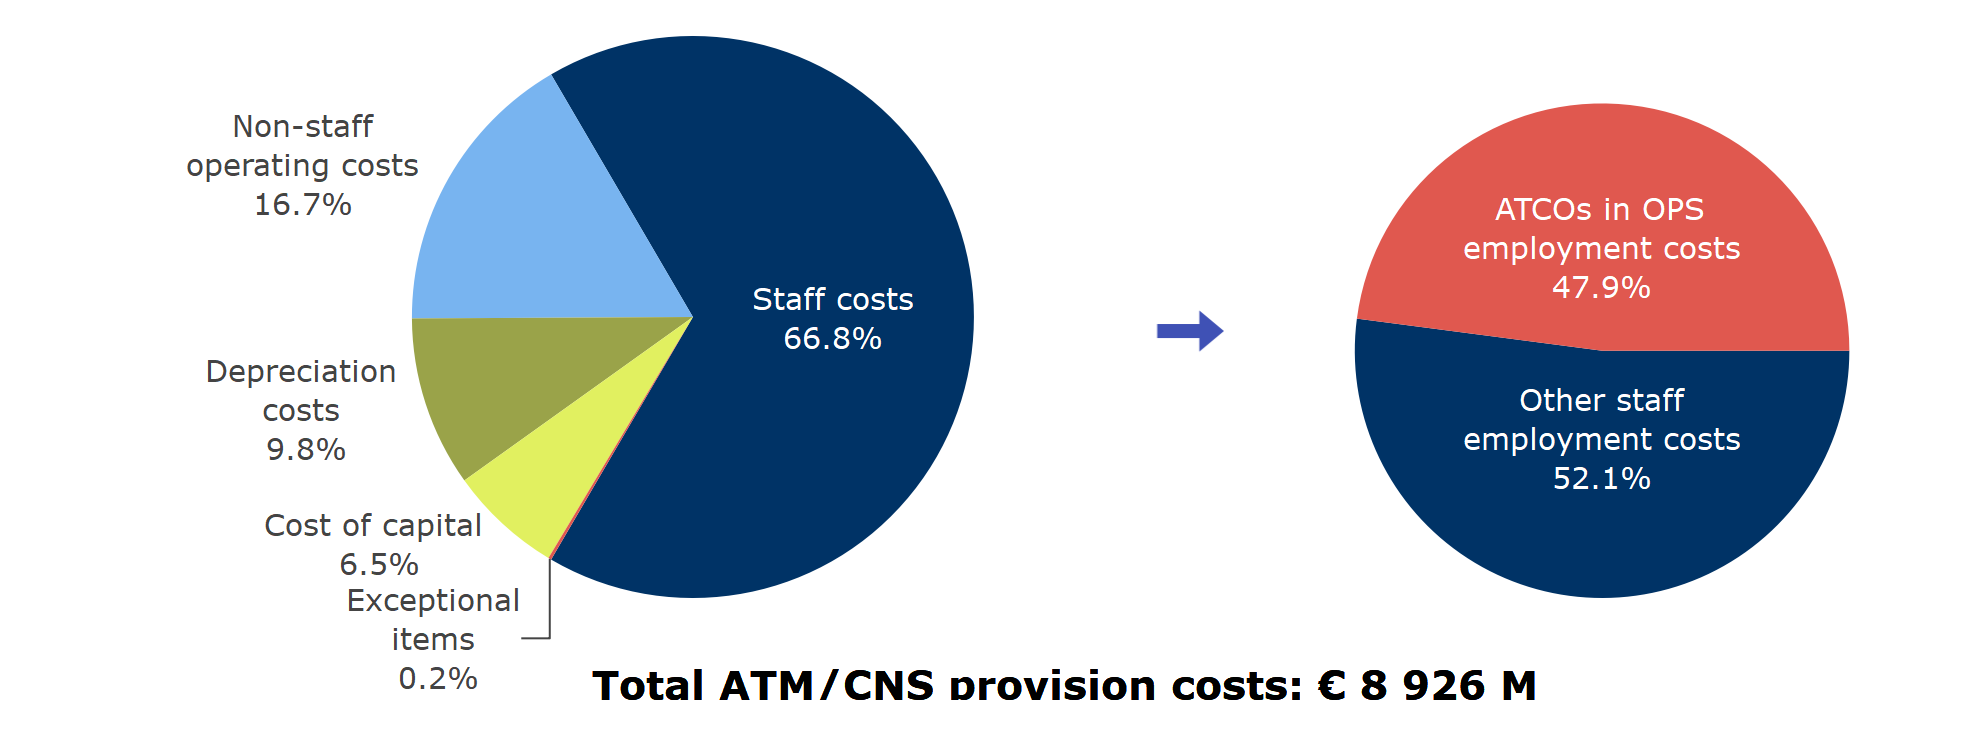
\includegraphics[width=1\textwidth,height=1\textheight]{figures/figure-2-3-hlsr_c_bdown_pie.png}

\newlength\holdLTleft\newlength\holdLTright\setlength\holdLTleft{\LTleft}\relax\setlength\holdLTright{\LTright}\relax\setlength\LTleft{0\linewidth}

\setlength\LTright{0\linewidth}

\begin{longtable*}{@{\extracolsep{\fill}}lrrrrrr}
\toprule
 & \multicolumn{2}{c}{En-route} & \multicolumn{2}{c}{Terminal} & \multicolumn{2}{c}{Gate-to-gate} \\ 
\cmidrule(lr){2-3} \cmidrule(lr){4-5} \cmidrule(lr){6-7}
  & € M & \% &  € M &  \% &   € M &   \% \\ 
\midrule\addlinespace[2.5pt]
Staff costs & 4 550 &  65.2\% & 1 275 &  65.4\% & 5 825 &  65.3\% \\ 
ATCOs in OPS employment costs & 2 229 & n.a. &   631 & n.a. & 2 859 & n.a. \\ 
Other staff employment costs     & 2 321 & n.a. &   644 & n.a. & 2 965 & n.a. \\ 
Non-staff operating costs & 1 155 &  16.6\% &   332 &  17.0\% & 1 487 &  16.7\% \\ 
Depreciation costs &   702 &  10.1\% &   172 &   8.9\% &   875 &   9.8\% \\ 
Cost of capital &   453 &   6.5\% &   129 &   6.6\% &   582 &   6.5\% \\ 
Exceptional items &   113 &   1.6\% &    40 &   2.0\% &   152 &   1.7\% \\ 
\cellcolor[HTML]{C0C0C0}{Total ATM/CNS provision costs} & \cellcolor[HTML]{C0C0C0}{6 973} & \cellcolor[HTML]{C0C0C0}{100.0\%} & \cellcolor[HTML]{C0C0C0}{1 948} & \cellcolor[HTML]{C0C0C0}{100.0\%} & \cellcolor[HTML]{C0C0C0}{8 921} & \cellcolor[HTML]{C0C0C0}{100.0\%} \\ 
\bottomrule
\end{longtable*}
\setlength\LTleft{\holdLTleft}
\setlength\LTright{\holdLTright}

}

\caption{\label{fig-figure-2-3}Gate-to-gate ATM/CNS provision costs at
Pan-European system level, 2022}

\end{figure}%

\begin{tcolorbox}[enhanced jigsaw, leftrule=.75mm, breakable, left=2mm, colframe=quarto-callout-note-color-frame, rightrule=.15mm, colback=white, opacityback=0, arc=.35mm, toprule=.15mm, bottomrule=.15mm]

\begin{figure}[H]

\begin{minipage}{0.35\linewidth}

\justifying \noindent \hfill\break \hfill\break After two years of
consecutive decreases, total ATM/CNS provision costs rose by +3.4\%
(+€296.8M) in 2022, reflecting cost increases for 26 out of 38 ANSPs.
Non-staff operating costs (+€118.8M) and the cost of capital (+€115.7M)
were the main sources of increase in 2022. The observed trend in the
cost of capital is heavily affected by a very large increase for
DHMI.\end{minipage}%
%
\begin{minipage}{0.65\linewidth}
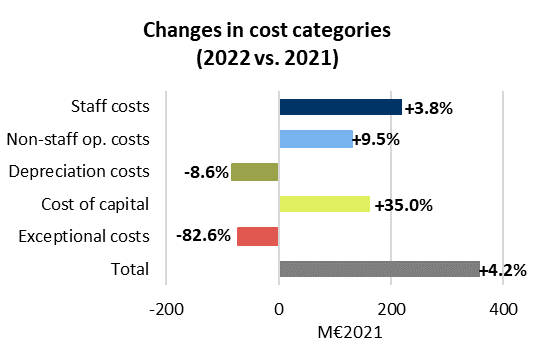
\includegraphics{figures/Figure-2-4.png}\end{minipage}%

\end{figure}%

\end{tcolorbox}

\newpage{}

In 2022, the five largest ANSPs (DFS, DSNA, ENAIRE, ENAV and NATS) bore
some 53\% of the total Pan-European gate-to-gate ATM/CNS provision
costs, while the five smallest ANSPs accounted for some 1\% (see bottom
left part of \textbf{?@fig-figure-2-5}).

\hfill\break
\begin{tightcenter}
\underline{Trends in ATM/CNS provision costs at Pan-European system level}
\end{tightcenter}

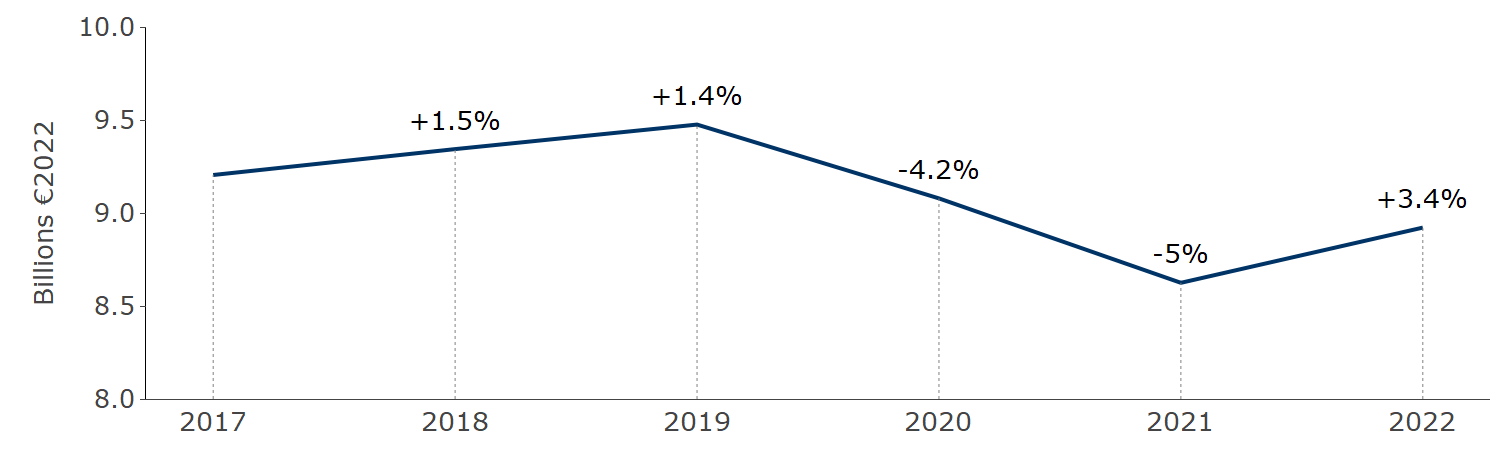
\includegraphics[width=0.85\textwidth,height=0.85\textheight]{figures/figure-2-5-1-hlsr_evo_cost.png}

\newpage{}

\begin{figure}

\centering{

\centering

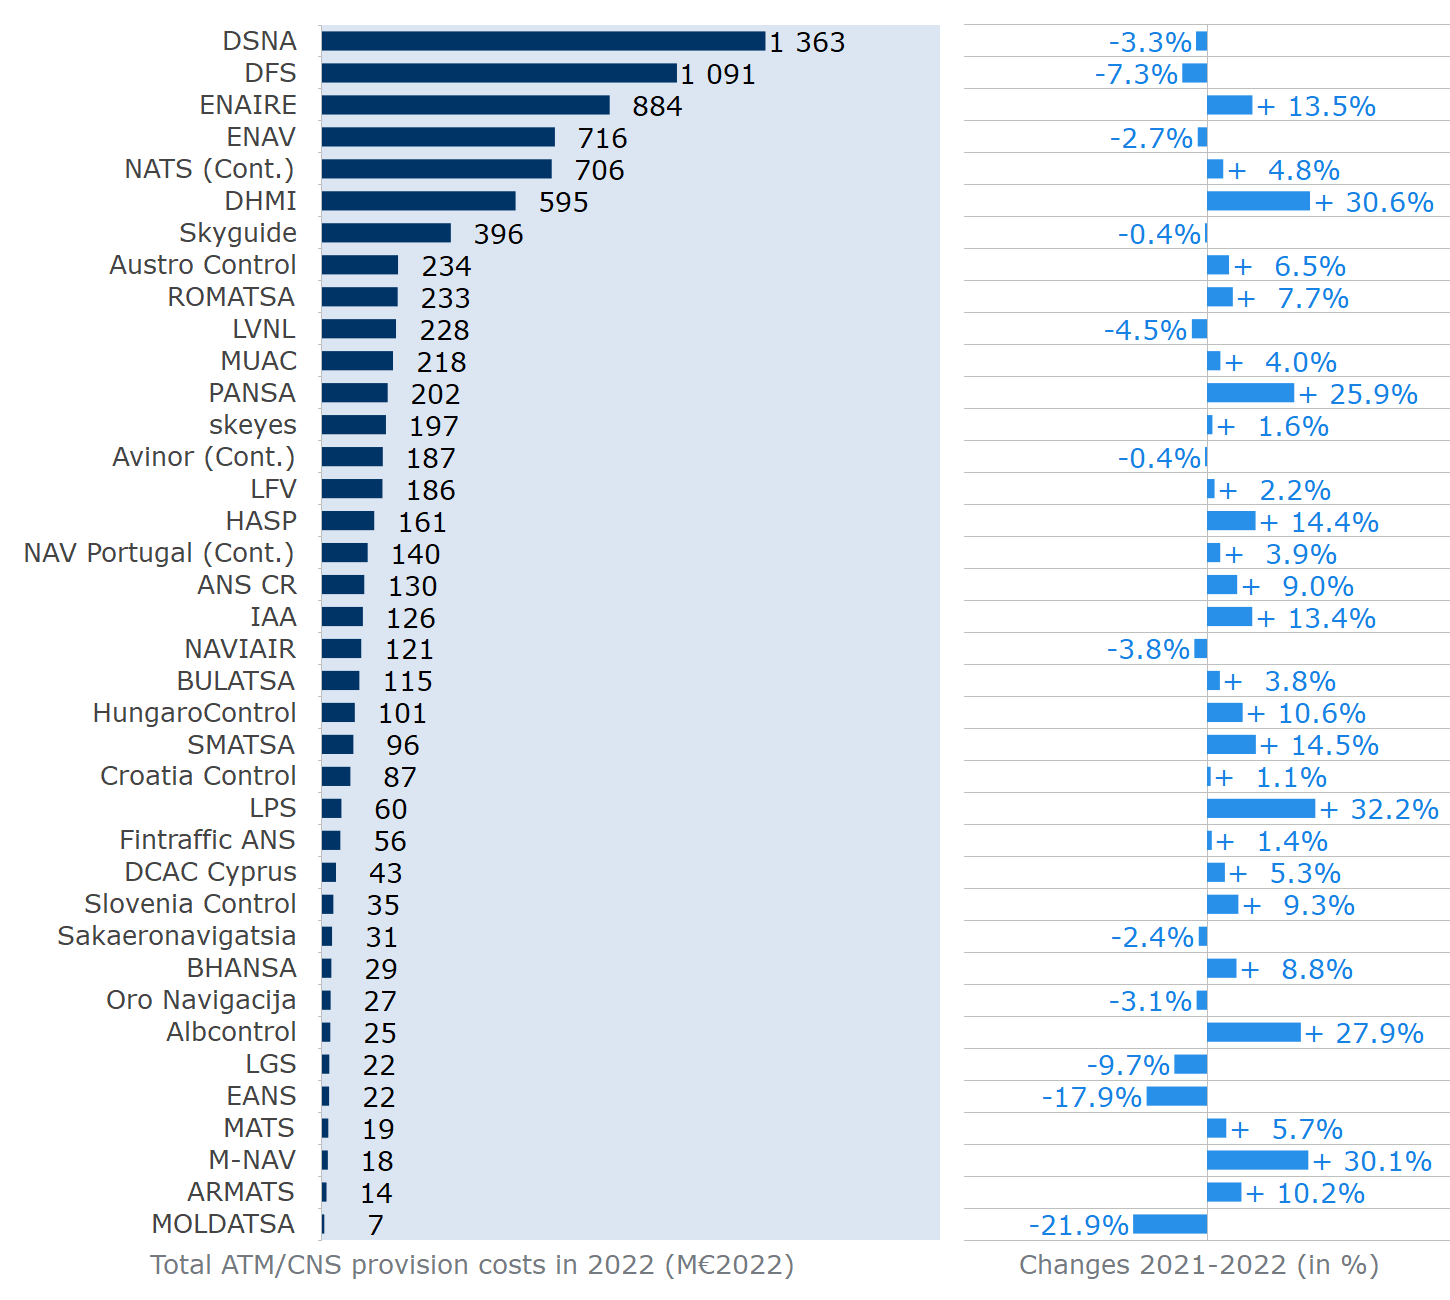
\includegraphics[width=0.79\textwidth,height=0.79\textheight]{figures/figure-2-5-23.png}

}

\caption{\label{fig-figure-2-5-2}Changes in ATM/CNS provision costs
(real terms)}

\end{figure}%

The Pan-European ANSPs employed a total of 52 497 staff in 2022
(comprising 51 680 staff providing ATM/CNS services and 817 internal MET
staff). Some 17 142 staff (33\%) were ATCOs working on operational
duties, split between ACCs (55\%) and APP/TWR facilities (45\%). On
average, 2.0 additional staff are required for every ATCO in OPS in
Europe.

\begin{figure}

\centering{

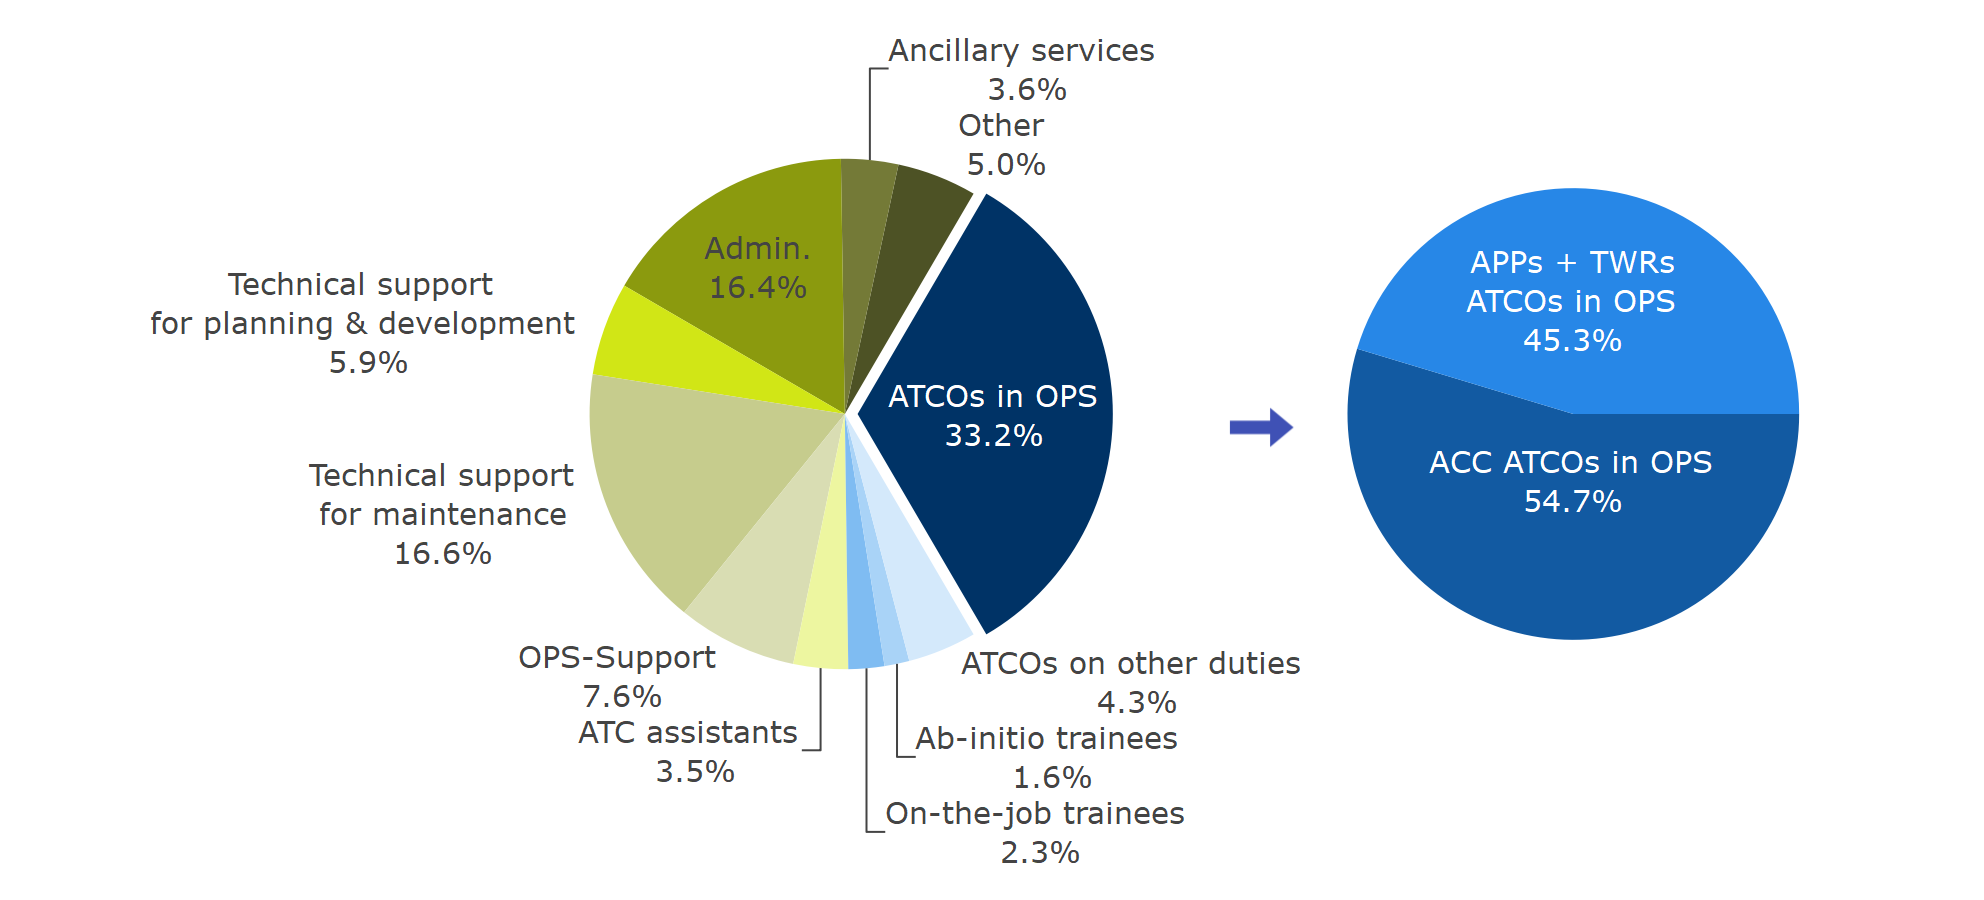
\includegraphics[width=0.93\textwidth,height=0.93\textheight]{figures/figure-2-6-hlsr_staff_pie.png}

}

\caption{\label{fig-figure-2-6}Breakdown of total gate-to-gate ATM/CNS
staff at Pan-European system level, 2022}

\end{figure}%

In 2022, the number of ATM/CNS staff was slightly lower than in 2021
(-0.9\% or -473 FTEs).

\newpage{}

\begin{tightcenter}
\hfill\break
\underline{Trends in gate-to-gate ATM/CNS staff at Pan-European system level}
\end{tightcenter}

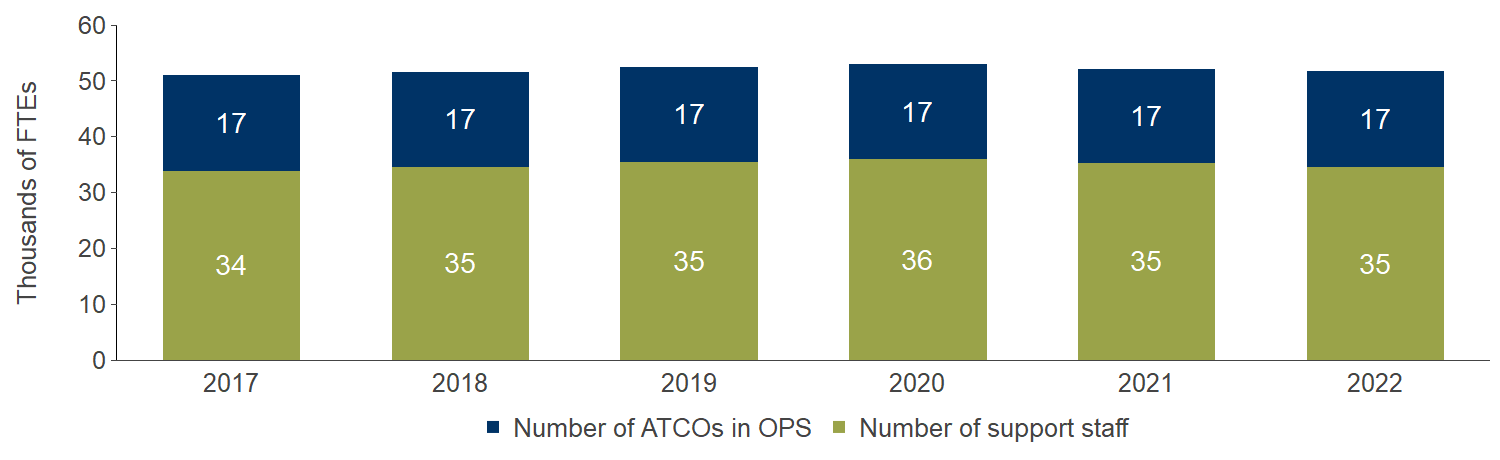
\includegraphics[width=0.9\textwidth,height=0.9\textheight]{figures/figure-2-7-1-hlsr_evo_staff.png}

\begin{figure}

\centering{

\centering

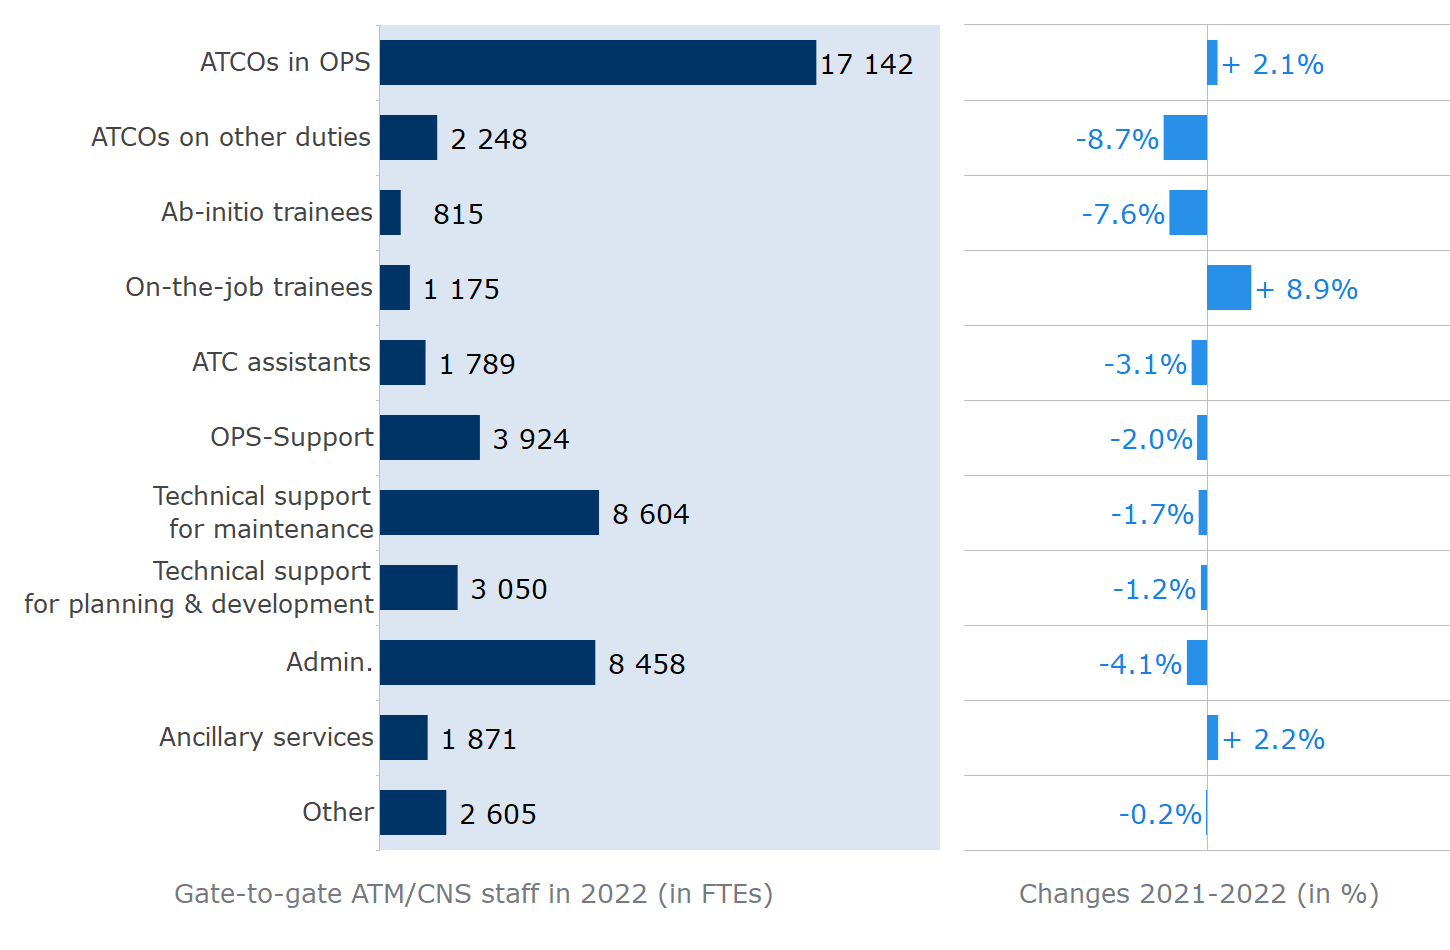
\includegraphics[width=0.85\textwidth,height=0.85\textheight]{figures/figure-2-7-23.png}

}

\caption{\label{fig-figure-2-7-2}Total gate-to-gate ATM/CNS staff per
staff category}

\end{figure}%

The overall change in staff numbers observed for 2022 mainly reflects
changes in the following staff categories:

\begin{itemize}
\tightlist
\item
  Administrative staff (-357 FTEs, or -4.1\%);
\item
  ATCOs in OPS (+356 FTEs, or +2.1\%); and,
\item
  ATCOs on other duties (-215 FTEs or -8.7\%).
\end{itemize}

To some extent, the changes observed for the ATCOs categories may
reflect the fact that some ATCOs previously reported as ``on other
duties'' following the traffic decrease in 2020 and the COVID-19
pandemic, are now re-allocated to OPS duties.

Decreases are also observed for technical support staff for operational
maintenance (-1.7\%), OPS support staff (-2.0\%), ab-initio trainees
(-7.6\%), ATC assistants (-3.1\%), technical support staff for planning
and development (-1.2\%) and other staff (-0.2\%). Conversely, the
number of on-the job trainees (+8.9\%) and staff for ancillary services
(+2.2\%) rose in 2022.

\bookmarksetup{startatroot}

\chapter{Economic cost-effectiveness}\label{sec-economic}

The concept of economic cost-effectiveness, developed by the PRC, is
defined as the sum of gate-to-gate ATM/CNS provision costs and the costs
of ground ATFM delays for both en‐route and airport, all expressed per
composite flight-hour. This economic performance indicator is meant to
capture trade‐offs between quality of service provided and
costs\footnote{See
  \url{https://ansperformance.eu/economics/ace/ace-handbook/} for more
  information on the methodology used to compute composite flight-hours
  and economic costs.}.

Figure~\ref{fig-figure-3-1} shows \ul{preliminary results} on the
changes in economic cost-effectiveness over 2017 - 2022 at Pan-European
system level. Figure~\ref{fig-figure-3-1-left} shows the changes in unit
economic costs, while Figure~\ref{fig-figure-3-1-right} provides
complementary information on the year-on-year changes in ATM/CNS
provision costs, composite flight-hours and unit costs of ATFM delays.
Unit economic costs significantly reduced in 2022 (-21.0\%). This
reduction results from the combination of a decrease in ATM/CNS
provision costs per composite flight-hour (-34.7\%) and a large increase
in the unit cost of ATFM delays (+325.3\%). Despite this large increase,
2022 unit costs remain +5.0\% higher than in 2019.

In 2022, ATFM delays increased almost six-fold to some 19.3M minutes. As
a result, the share of ATFM delays in the 2022 unit economic costs
amounts to 20\%. This is close to the level reached in 2019, which was a
year marked by significant capacity issues for several ANSPs.

\begin{figure}[h]

\begin{minipage}{0.50\linewidth}

\centering{

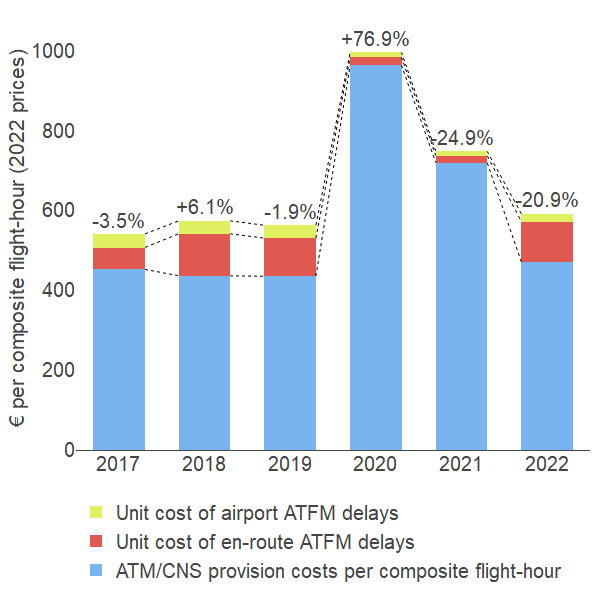
\includegraphics{figures/figure-3-1-1-hlsr_evo_eco_ce.png}

}

\subcaption{\label{fig-figure-3-1-left}~}

\end{minipage}%
%
\begin{minipage}{0.50\linewidth}

\centering{

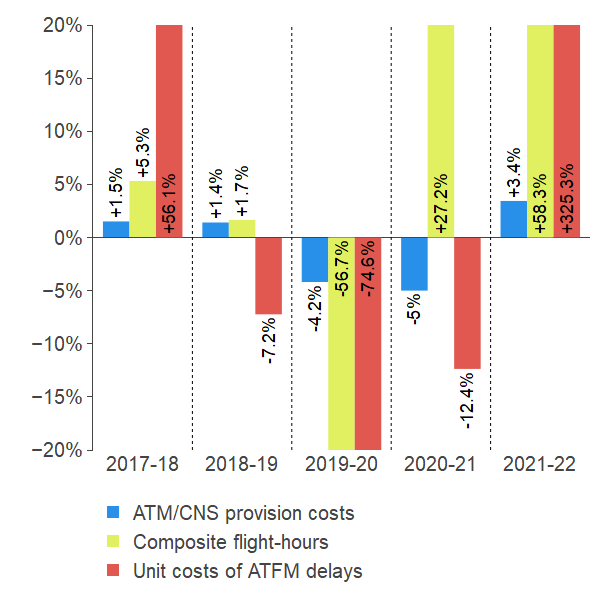
\includegraphics{figures/figure-3-1-2-hlsr_evo_eco_ce_comp.png}

}

\subcaption{\label{fig-figure-3-1-right}~}

\end{minipage}%

\caption{\label{fig-figure-3-1}Trend of unit economic costs at
Pan-European system level, 2017-2022 (real terms)}

\end{figure}%

Figure~\ref{fig-figure-3-2} shows \ul{preliminary results} at ANSP level
(dotted lines represent the 1st and 3rd quartiles, €411 and €635,
respectively).

\begin{figure}[h]

\centering{

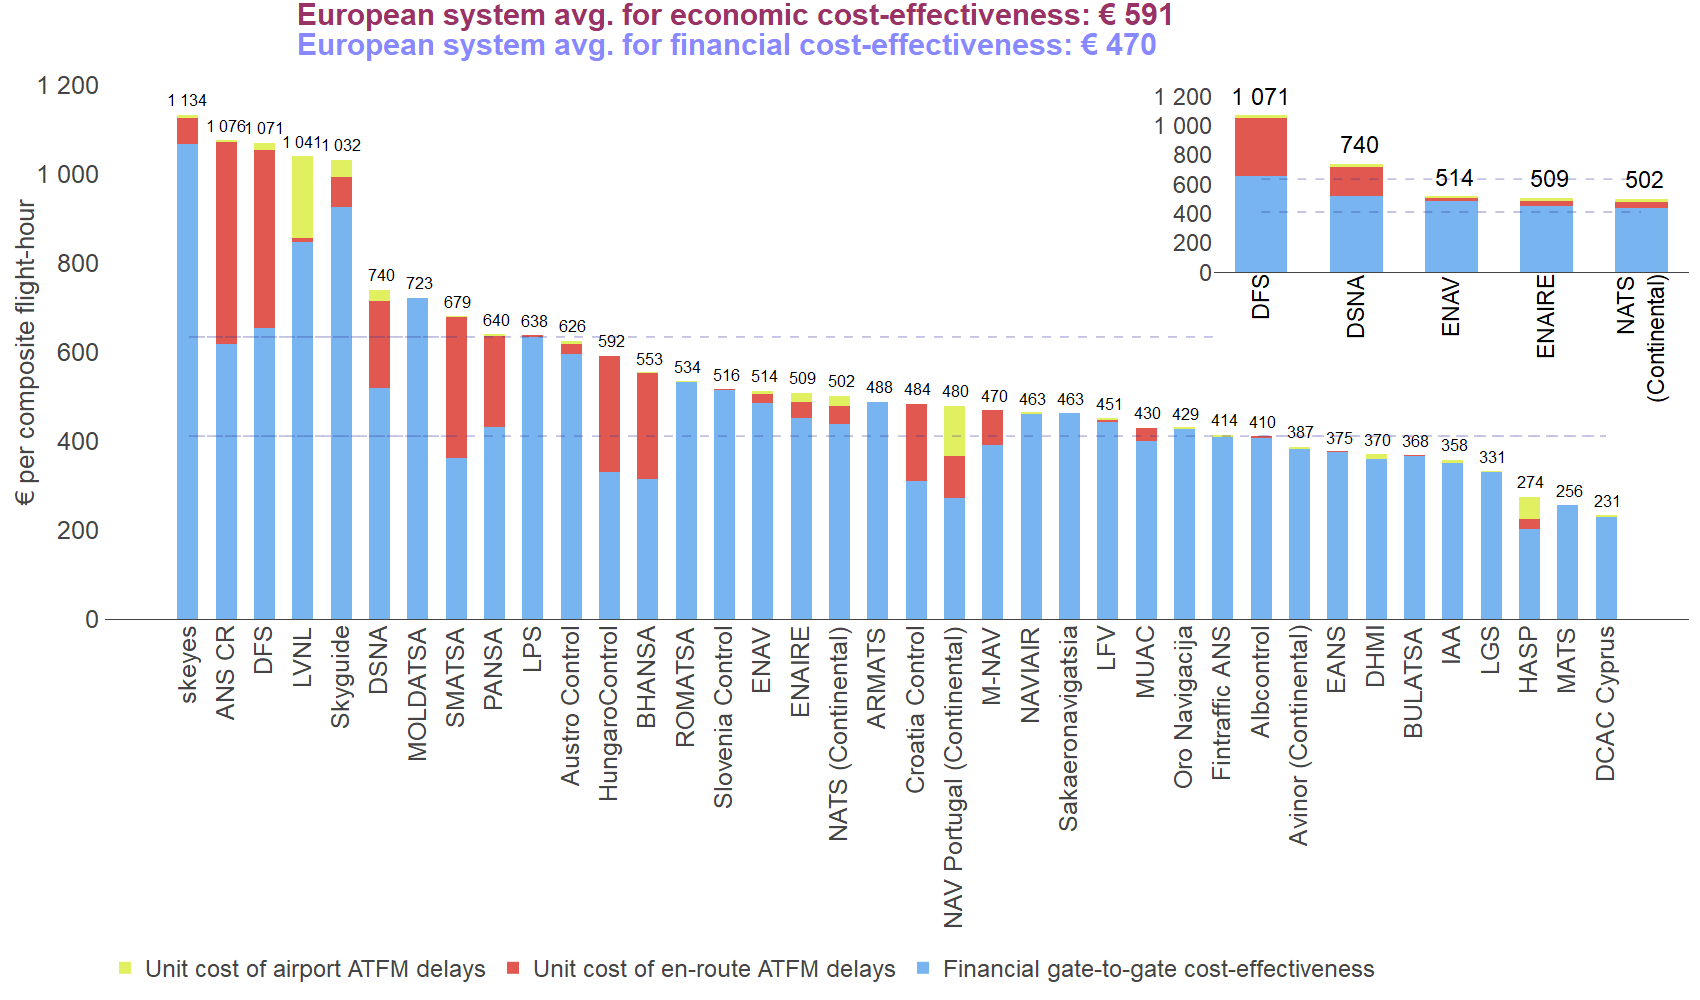
\includegraphics{figures/figure-3-2-hlsr_eco_ce.png}

}

\caption{\label{fig-figure-3-2}Economic gate-to-gate cost-effectiveness,
2022 }

\end{figure}%

\vspace{14cm}

For ten ANSPs ATFM delays represented more than 20\% of their unit
economic costs (see ANSPs with the largest red and lime portions,
e.g.~ANS CR, DFS, SMATSA, HungaroControl, etc.). In absolute terms
(cumulative ATFM delays in minutes), DFS, DSNA, ENAIRE, NAV Portugal and
NATS were the ANSPs generating the highest levels of ATFM delays in 2022
(70\% of the pan-European system total ATFM delays). For some of these
ANSPs, work associated with the implementation of new ATM systems caused
a temporary reduction of the available capacity and as a consequence
contributed to increase ATFM delays (this was for example the case for
DSNA and NAV Portugal). Other ANSPs, for example PANSA, were affected by
airspace closure due to extended monitoring activities performed by the
military at the border with Ukraine, due to the ongoing war therein.

Further analysis of the relationship between changes in ANSPs costs,
traffic and unit costs will be analysed in detail in the forthcoming ACE
report.

\bookmarksetup{startatroot}

\chapter{Financial cost-effectiveness}\label{sec-financial}

This chapter provides a \ul{preliminary analysis} of financial
cost-effectiveness.

\section{Pan-European system level}\label{sec-fin_1}

Figure~\ref{fig-figure-4-1} shows that in 2022 the unit ATM/CNS
provision costs fell by -34.7\% compared to 2021, reaching an amount of
€470. This is the result of traffic increase (+58.3\%) coupled with the
growth of ATM/CNS provision costs (+3.4\%).

However, Comparing with pre-pandemic levels, in 2022 unit ATM/CNS
provision costs still remain +8.2\% higher than in 2019. This mainly
reflects the fact that, despite a lower cost-base (-6.1\% compared to
2019) traffic volumes in 2022 still did not reach the 2019 level
(-13.3\%).

\begin{figure}

\centering{

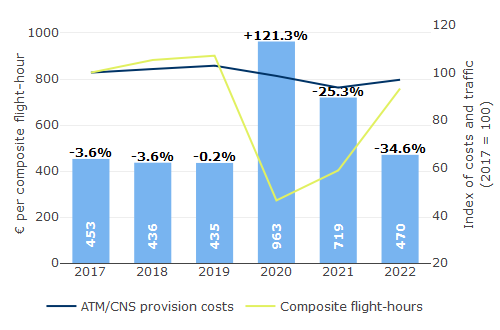
\includegraphics[width=0.75\textwidth,height=0.75\textheight]{figures/figure-4-1-hlsr_evo_unit_cost.png}

}

\caption{\label{fig-figure-4-1}Changes in unit ATM/CNS provision costs,
2017 -- 2022 (real terms)}

\end{figure}%

The analytical framework used in the ACE analysis to break down the
financial cost-effectiveness indicator into relevant economic drivers is
presented in Figure~\ref{fig-figure-4-2}. These key drivers include:

a) ATCO-hour productivity (0.88 composite flight-hours per ATCO-hour);

b) ATCO employment costs per ATCO-hour (€133); and,

c) support costs per unit output (€319).

\newpage{}

\begin{figure}

\centering{

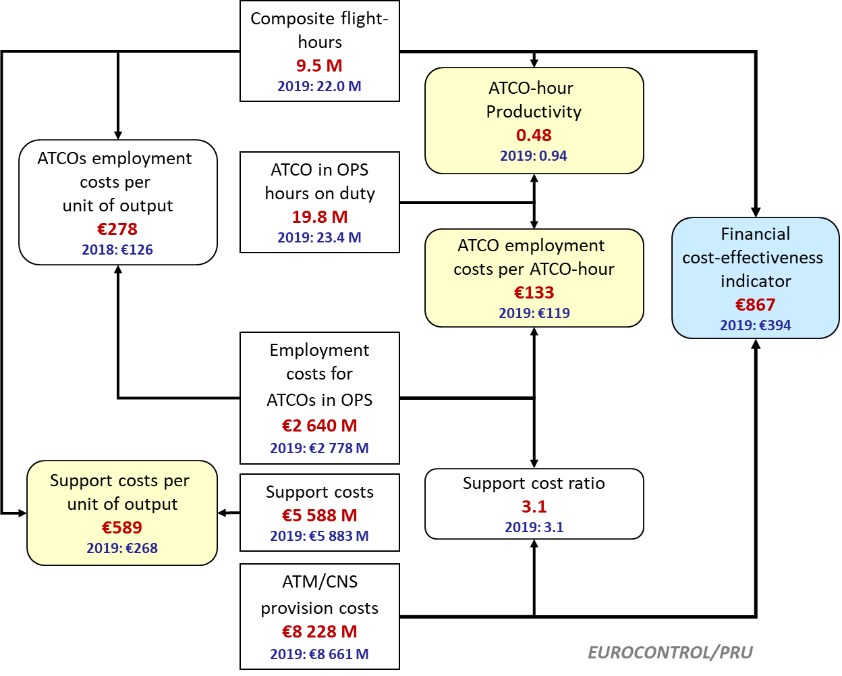
\includegraphics[width=0.88\textwidth,height=0.88\textheight]{figures/Figure-4-2.png}

}

\caption{\label{fig-figure-4-2}ACE performance framework, 2022 (real
terms)}

\end{figure}%

Figure~\ref{fig-figure-4-3} shows that in 2022, ATCO employment costs
per ATCO-hour fell by -2.3\% while ATCO-hour productivity rose by
+46.9\%. As a result, ATCO employment costs per composite flight-hour
decreased (-33.5\%). In the meantime, unit support costs fell by -35.2\%
due to the combination of an increase in composite flight-hours
(+58.3\%) and an increase in support costs (+2.6\%). As a result, in
2022, unit ATM/CNS provision costs fell by -34.7\% at Pan-European
system level.

\begin{figure}

\centering{

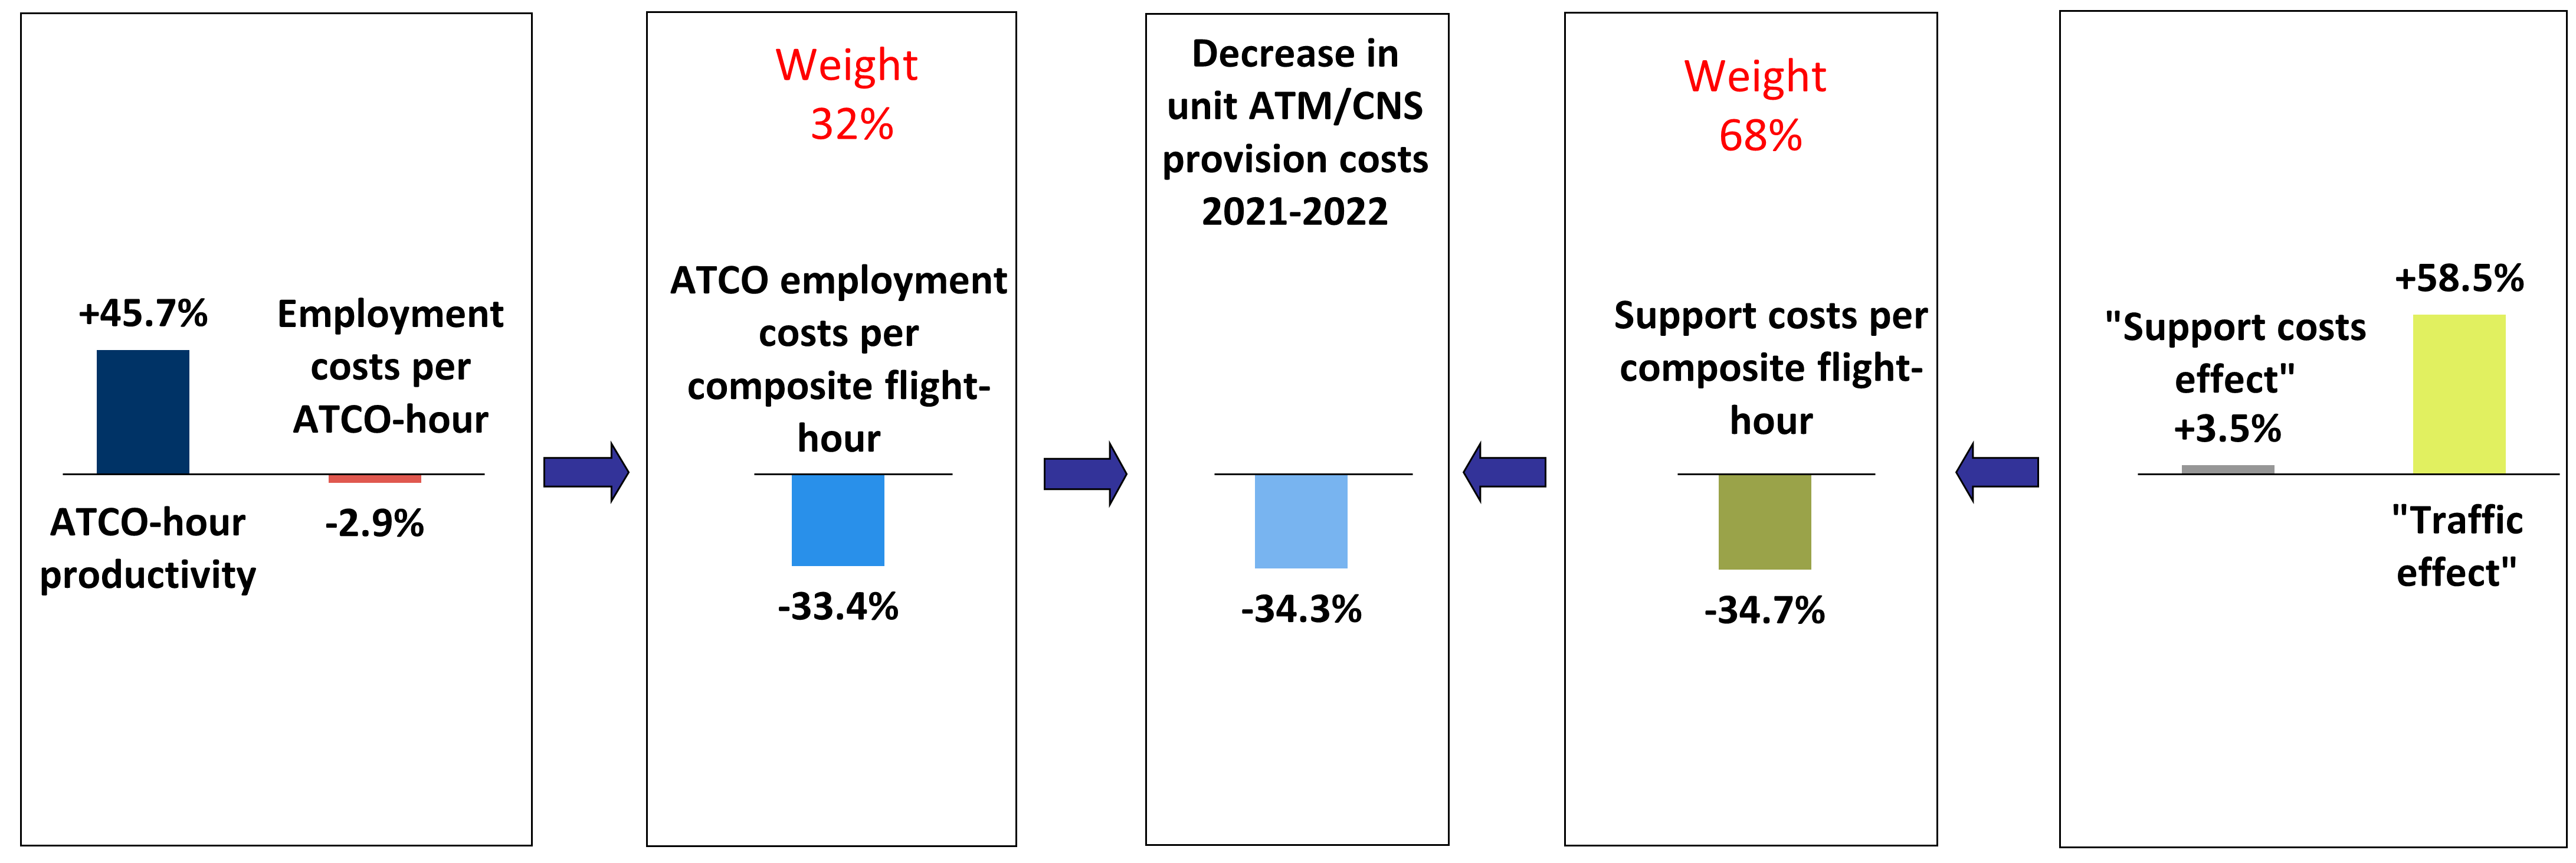
\includegraphics[width=0.98\textwidth,height=0.98\textheight]{figures/Figure-4-3.png}

}

\caption{\label{fig-figure-4-3}Breakdown of changes in unit ATM/CNS
provision costs, 2021 -- 2022 (real terms)}

\end{figure}%

As the values of the 2021 indicators were significantly affected by the
consequences of the COVID-19 crisis, Figure~\ref{fig-figure-4-3-2} below
provides an additional analysis using 2019 as a reference year. It shows
that in 2022 the traffic was still well below its 2019 level and,
despite a reduction in total support costs, the unit support costs were
higher than in 2019. A similar situation is observed on the ATCO
employment costs side where the reduction in employment costs per
ATCO-hour was not sufficient to compensate for the decrease in ATCO-hour
productivity. Overall, the unit cost in 2022 was then +8.2\% higher than
in 2019.

\begin{figure}

\centering{

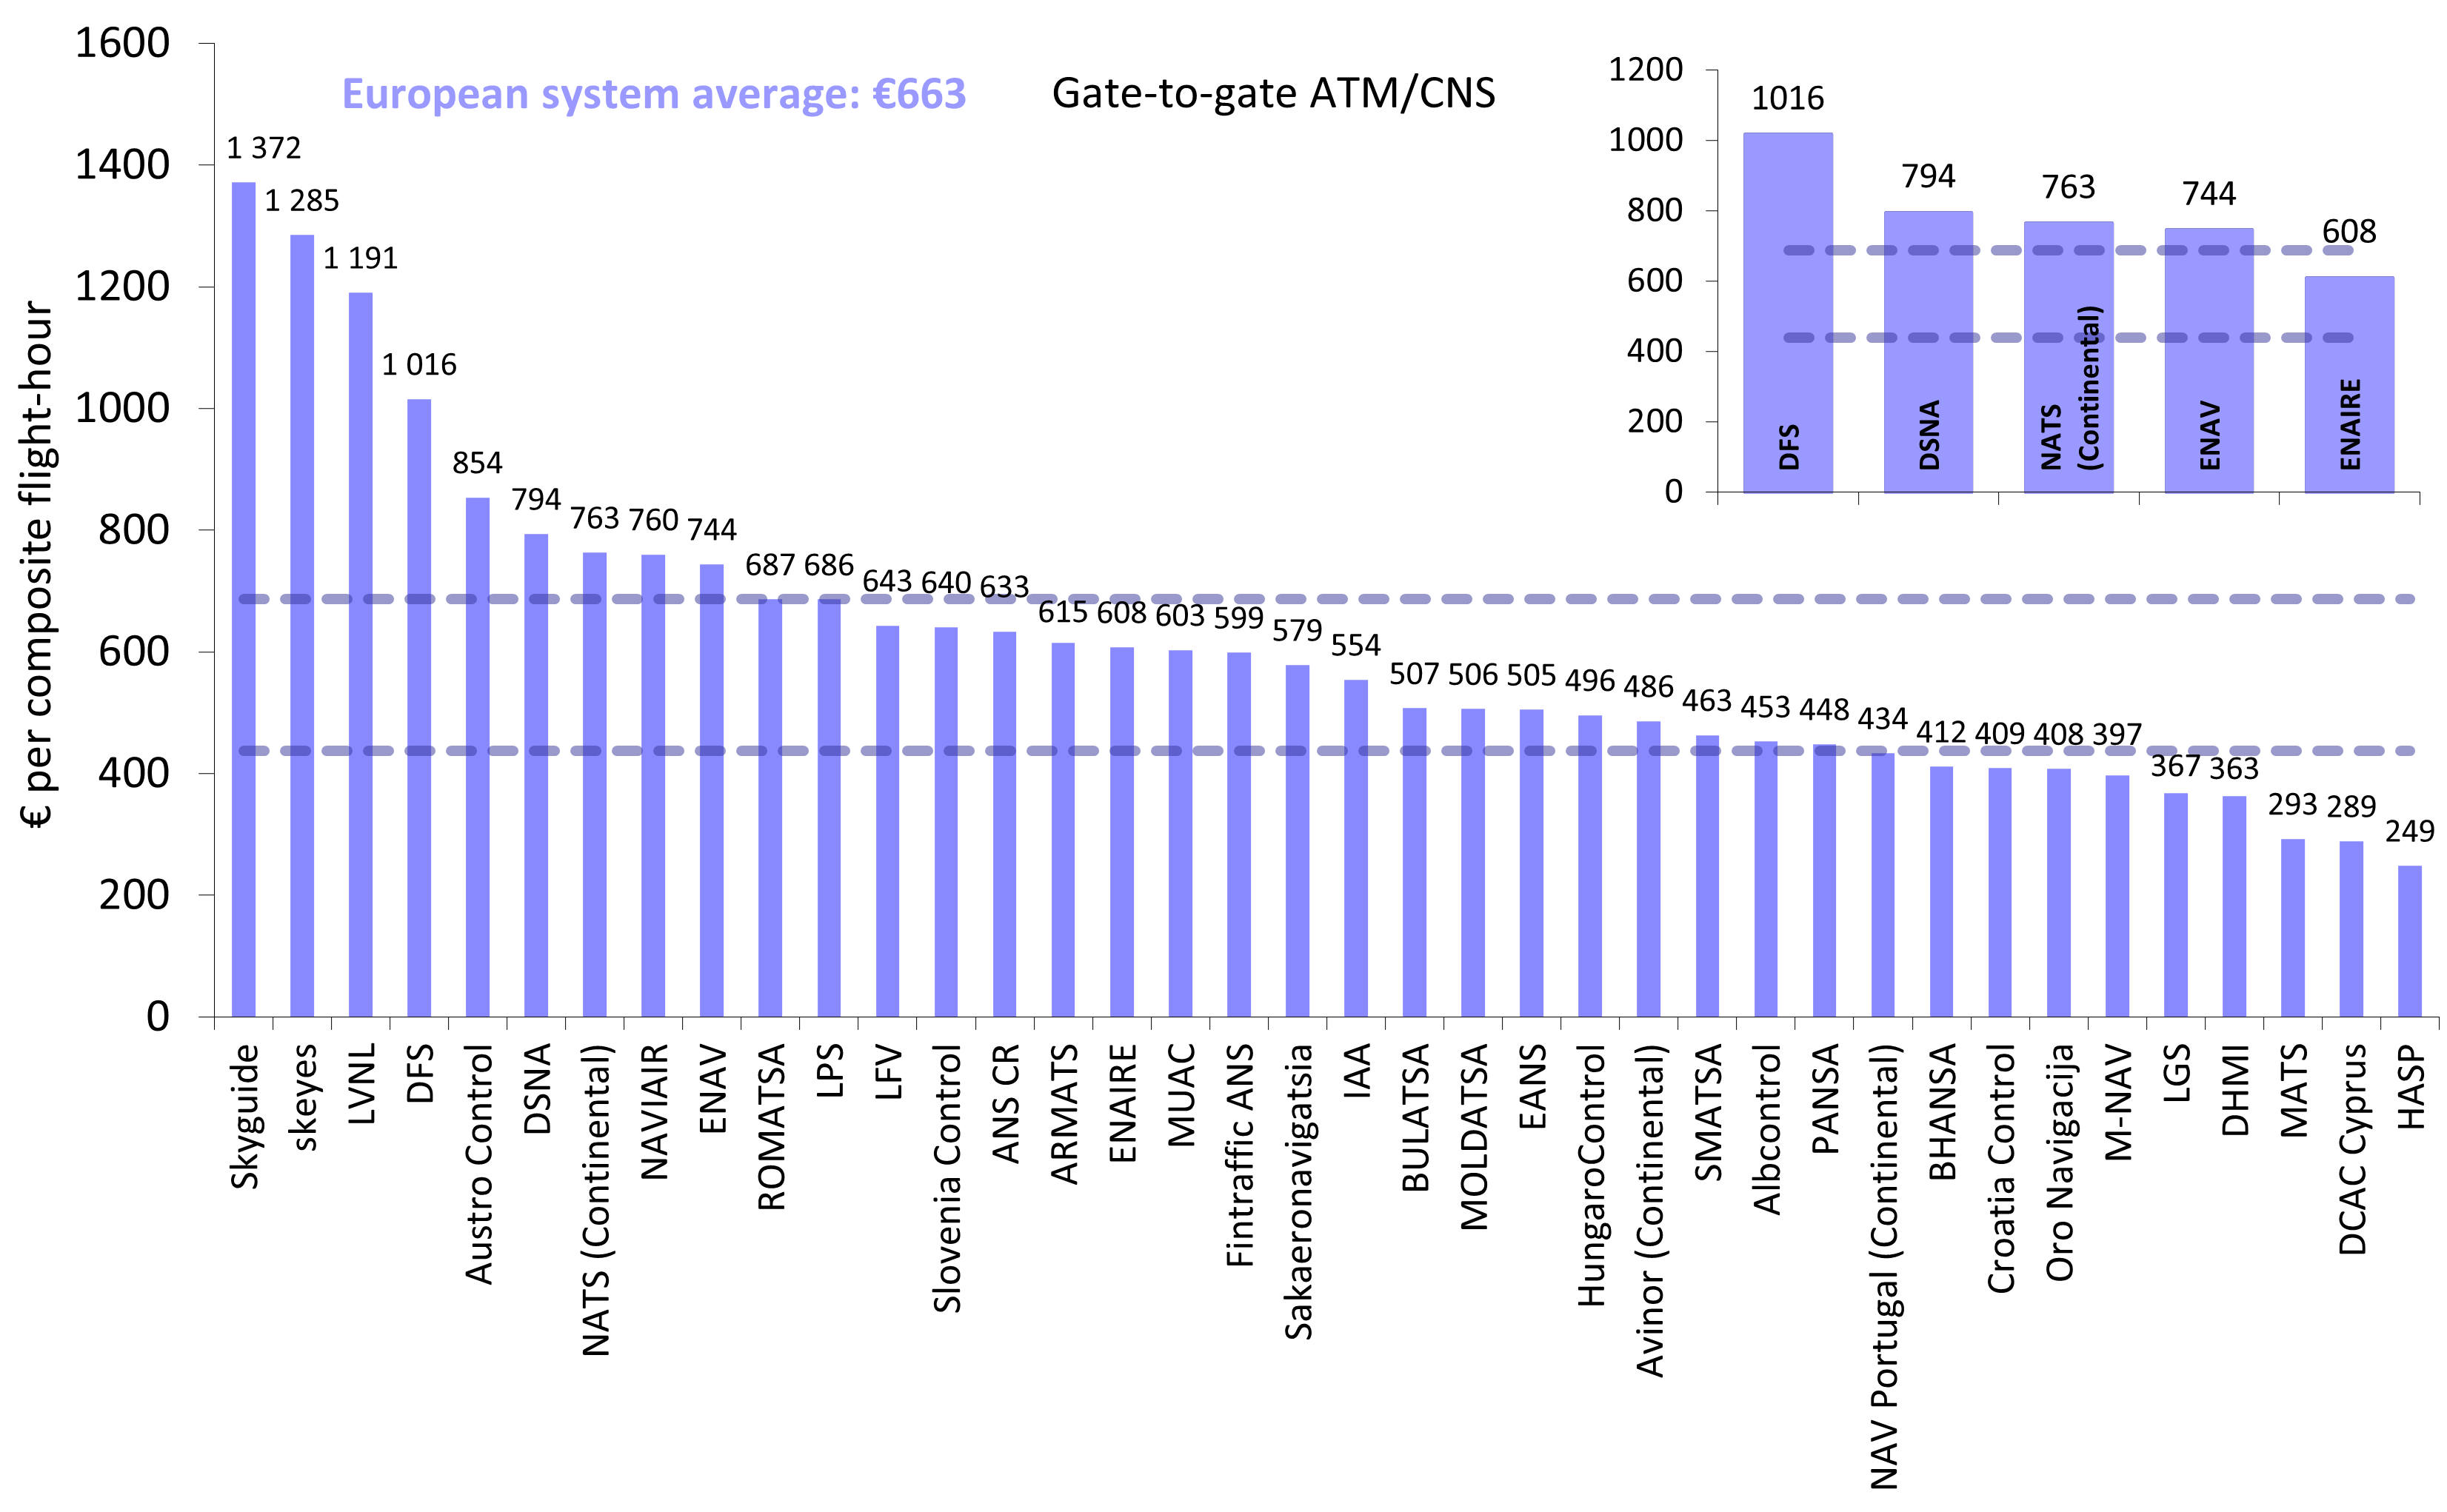
\includegraphics[width=0.98\textwidth,height=0.98\textheight]{figures/Figure-4-4.png}

}

\caption{\label{fig-figure-4-3-2}Breakdown of changes in unit ATM/CNS
provision costs, 2019 -- 2022 (real terms)}

\end{figure}%

\newpage{}

\section{ANSP level}\label{sec-fin_2}

All figures presented in this section present the preliminary
benchmarking results for the 38 ANSPs. Because of their weight in the
Pan-European system and their relatively similar operational and
economic characteristics, the five largest ANSPs (DFS, DSNA, ENAIRE,
ENAV and NATS) are also shown in a miniature replica of the chart (top
right corner of the figures). The 1st and 3rd quartiles for each
indicator are also shown in all figures. The gap between these two
quartiles provides additional insight on the dispersion of the values.

Figure~\ref{fig-figure-4-4} presents the financial gate-to-gate
cost-effectiveness indicator at ANSP level for the year 2022. The dotted
lines represent the 1st and 3rd quartiles (€360 and €518, respectively).

\hfill\break

\begin{figure}[h]

\centering{

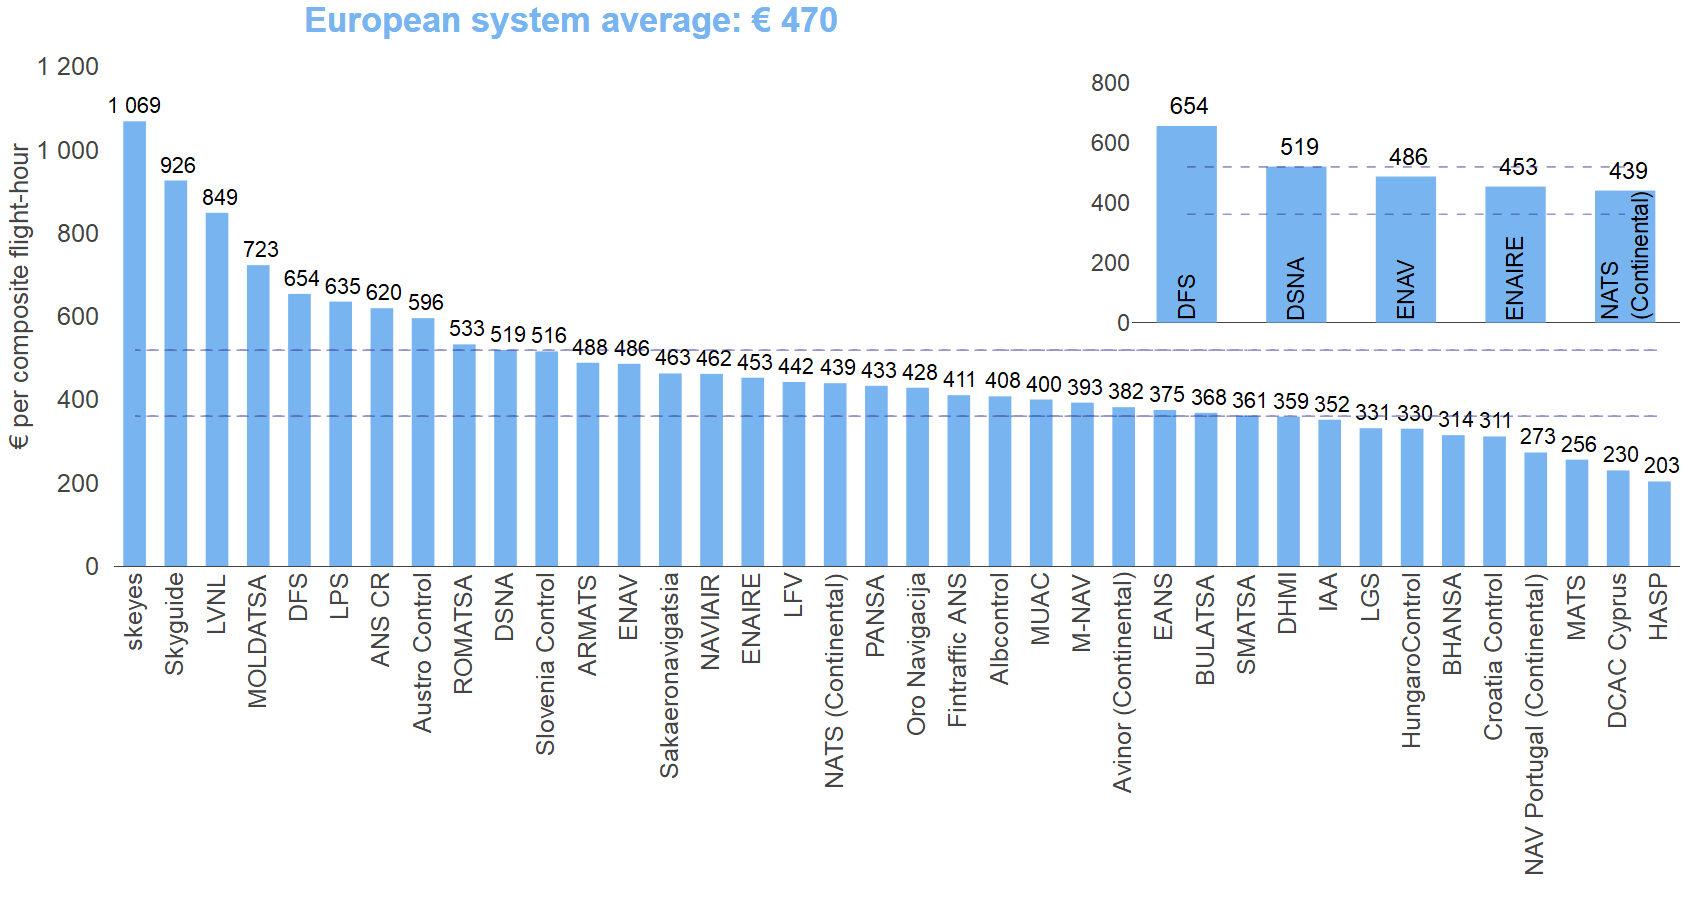
\includegraphics{figures/figure-4-4-hlsr_fin_ce.png}

}

\caption{\label{fig-figure-4-4}Financial gate-to-gate
cost-effectiveness, 2022}

\end{figure}%

\newpage{}

Figure~\ref{fig-figure-4-5} presents the ATCO-hour productivity
indicator at ANSP level for the year 2022. The dotted lines represent
the 1st and 3rd quartiles (0.61 and 0.93, respectively).

\hfill\break

\begin{figure}[h]

\centering{

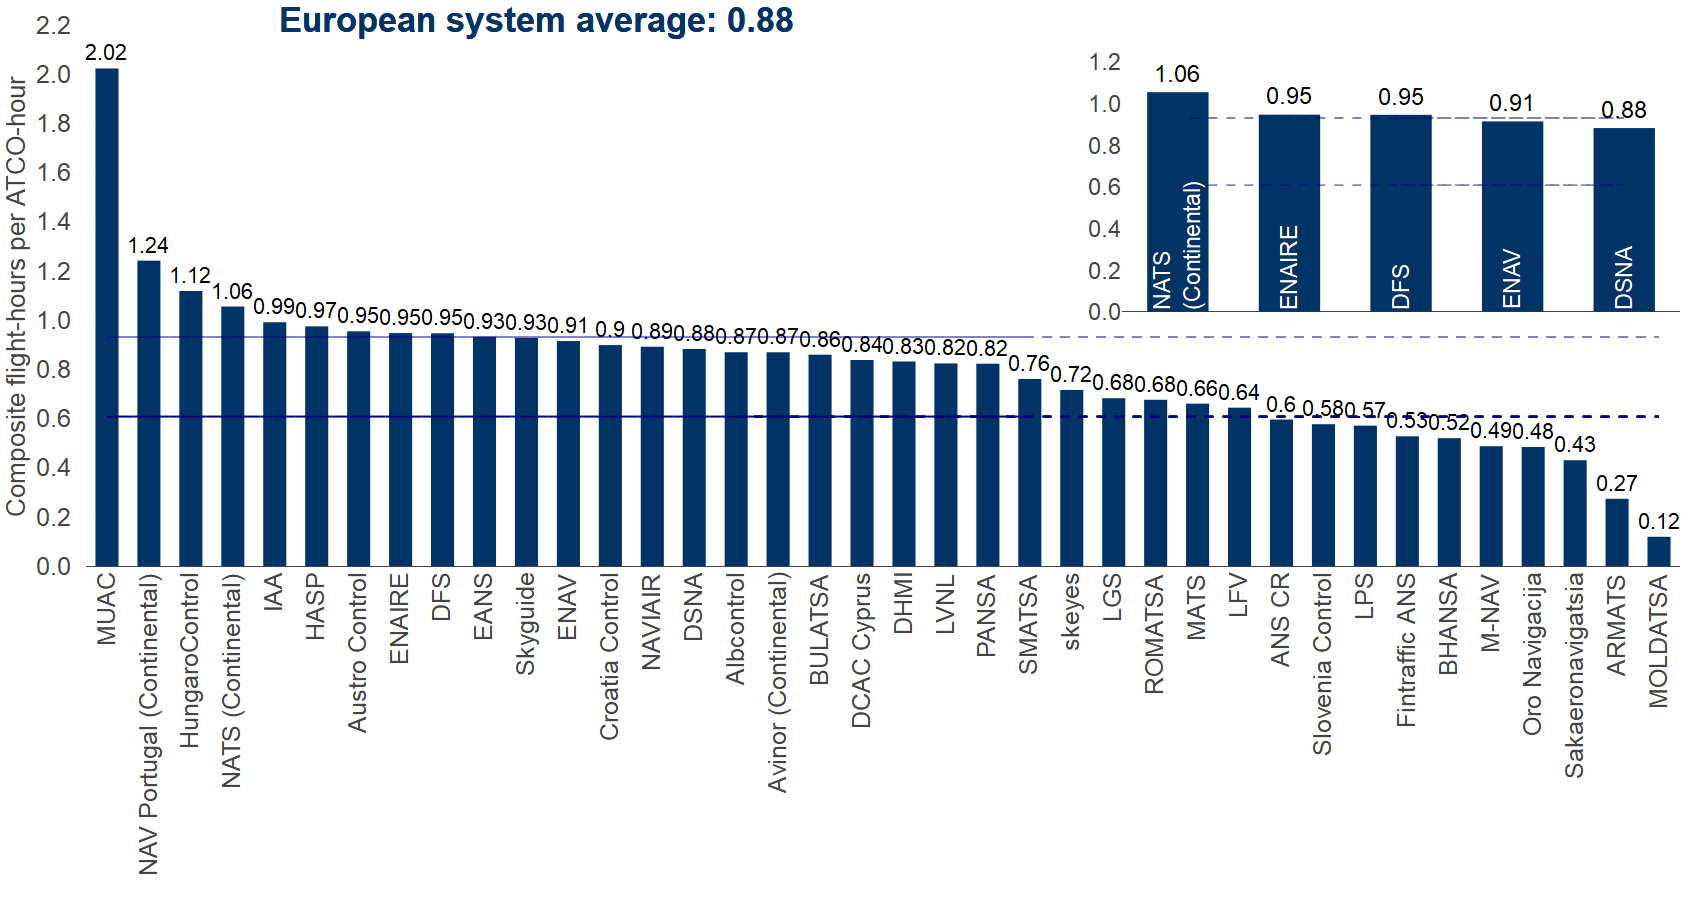
\includegraphics{figures/figure-4-5-hlsr_prod.png}

}

\caption{\label{fig-figure-4-5}ATCO-hour productivity, 2022}

\end{figure}%

Figure~\ref{fig-figure-4-6} presents the employment costs per ATCO in
OPS indicator at ANSP level for the year 2022. The dotted lines
represent the 1st and 3rd quartiles (€58 and €141, respectively).

\hfill\break

\begin{figure}[h]

\centering{

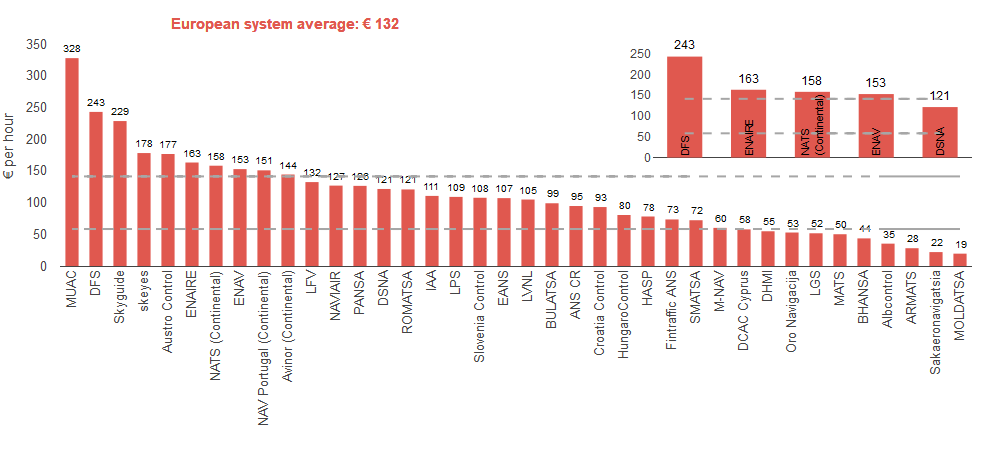
\includegraphics{figures/figure-4-6-hlsr_atco_cost_h.png}

}

\caption{\label{fig-figure-4-6}Employment costs per ATCO-hour, 2022}

\end{figure}%

\newpage{}

Figure~\ref{fig-figure-4-7} presents the support costs per composite
flight-hour indicator at ANSP level for the year 2022. The dotted lines
represent the 1st and 3rd quartiles (€243 and €382, respectively).

\hfill\break

\begin{figure}[h]

\centering{

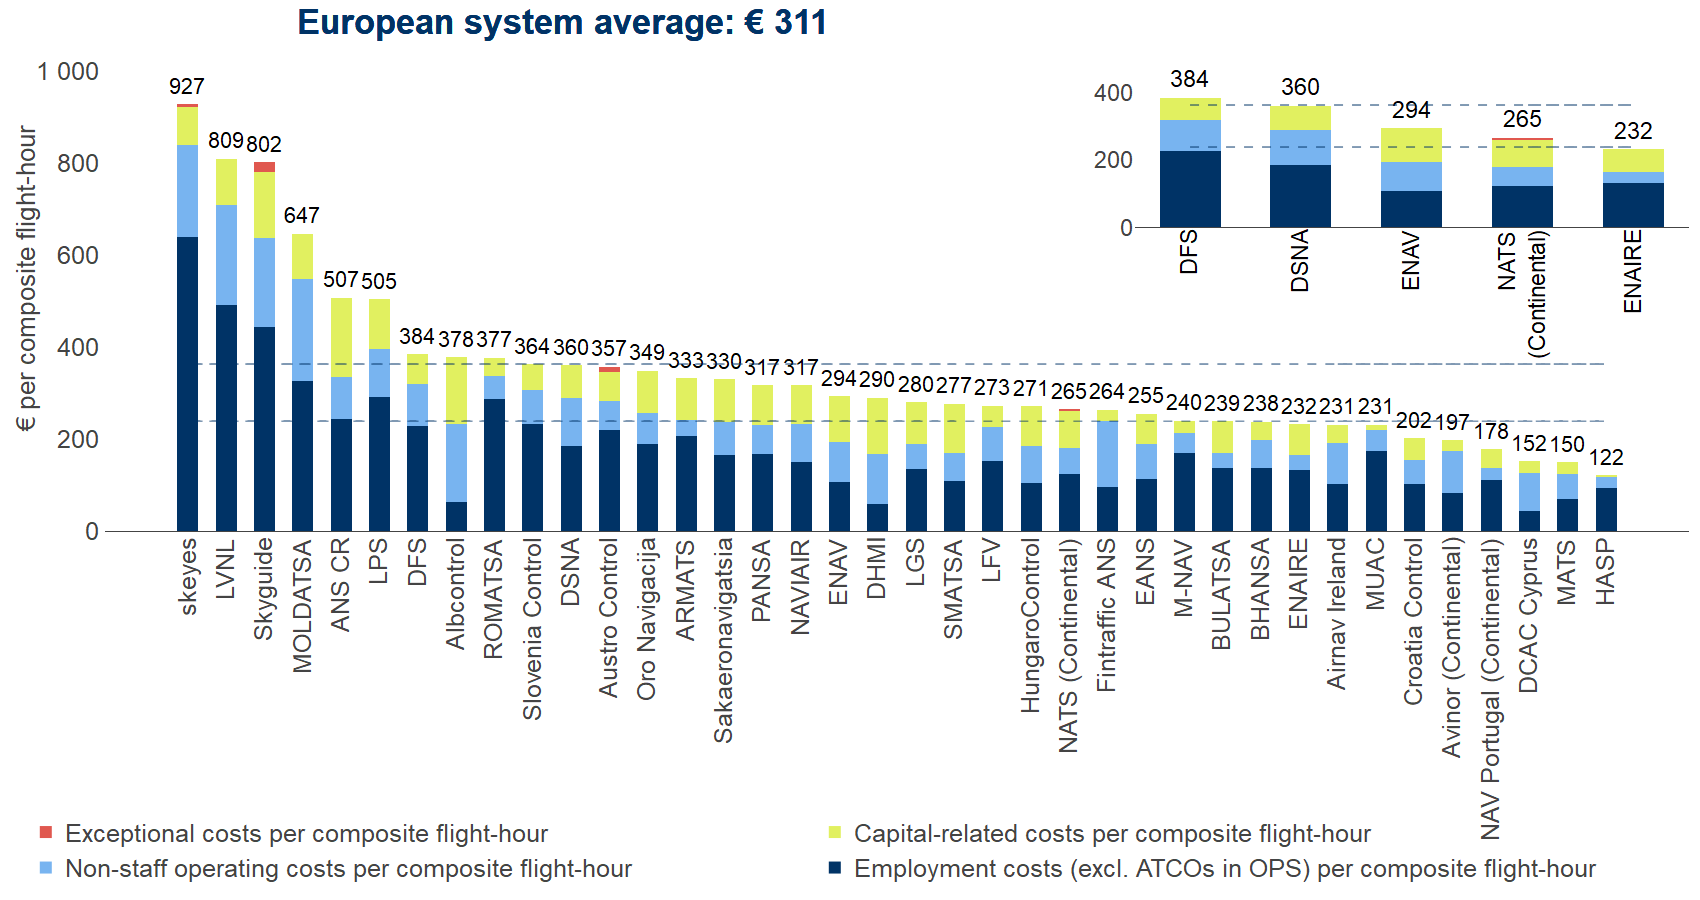
\includegraphics{figures/figure-4-7-hlsr_support.png}

}

\caption{\label{fig-figure-4-7}Breakdown of support costs per composite
flight-hour, 2022}

\end{figure}%

A more detailed analysis of the changes in cost-effectiveness, ATCO-hour
productivity, ATCO employment costs per ATCO-hour and unit support costs
will be available in the final ACE benchmarking report.

\bookmarksetup{startatroot}

\chapter{Monitoring of ANSPs cash and liquidity
situation}\label{sec-covid}

This chapter provides an overview of ANSPs' financial situation over the
2017 - 2022 period, using two indicators: the current ratio and the
cash-on-hand days. These indicators have been calculated at pan-European
system level using the information provided in the ANSPs' Financial
Statements which were available at the time of publishing this report
(34 for the 2017-2021 period and 23 in 2022). The indicators are
therefore consistent with those published at individual ANSP level in
the EUROCONTROL Aviation Intelligence Unit
\href{https://ansperformance.eu/economics/finance/}{ANSPs Financial
Dashboard}.

Depending on the organisational set up of different ANSPs, the
information reported in their financial statements covers a different
scope of activities (e.g.~it may include airport management operations,
commercial activities, etc.) which does not always correspond with the
ACE gate-to-gate scope. Additionally, due to specific organisational and
financial set up, DCAC Cyprus, HASP, LVNL and MUAC, are excluded from
the analysis presented in this chapter.

Figure~\ref{fig-figure-5-1} presents the changes in the average current
ratio between 2017 and 2022 as well as the 1st and 3rd quartiles. The
current ratio (current assets divided by current liabilities) measures
the ability of a company to pay its short-term debt obligations with its
current assets. On average, the situation slightly improved in 2022
following four years of continuous deterioration. However, for 25\% of
the sample, the current ratio has shown only small improvement since
reaching its lowest level in 2020.

\begin{figure}

\centering{

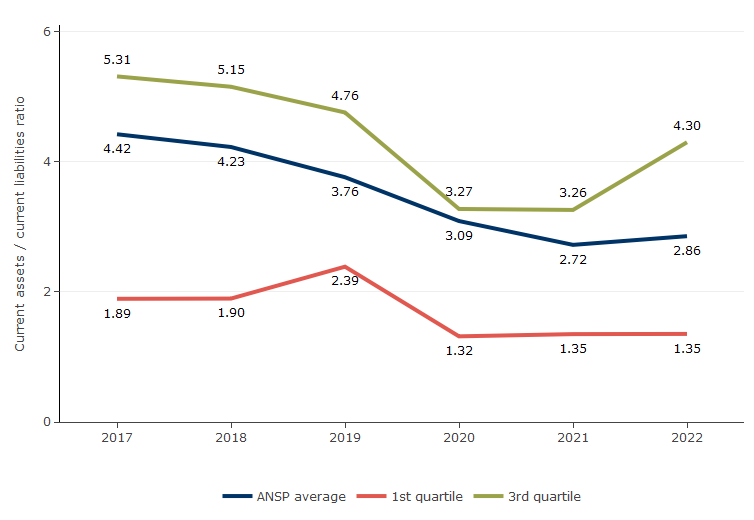
\includegraphics[width=0.85\textwidth,height=0.85\textheight]{figures/figure-5-1-hlsr_current_ratio.png}

}

\caption{\label{fig-figure-5-1}Trends in ANSPs current ratio 2017 -
2022}

\end{figure}%

Figure~\ref{fig-figure-5-2} shows the changes in cash-on-hand days at
Pan-European system level over the 2017 - 2022 period as well as the 1st
quartile and the 3rd quartile of these indicators. The cash-on-hand days
indicator (cash \& cash equivalents divided by operating costs x 365)
measures the length of time a company can pay its operating costs from
its cash reserves.

\newpage{}

\begin{figure}

\centering{

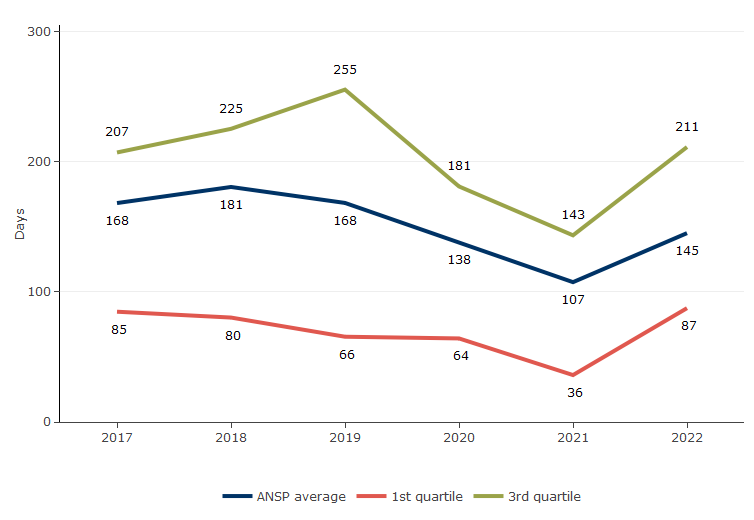
\includegraphics[width=0.85\textwidth,height=0.85\textheight]{figures/figure-5-2-hlsr_cash_on_hand.png}

}

\caption{\label{fig-figure-5-2}2017 - 2022 trends in cash-on-hand days
at Pan-European system level}

\end{figure}%

In 2022, the average cash-on-hand days amounted to 172 days, which is
+65 days higher than in 2021 and +34 days higher than in 2020. The 2022
figure reached the pre-pandemic levels. More detailed analysis on these
financial indicators will be available in the forthcoming ACE report.

\bookmarksetup{startatroot}

\chapter*{Disclaimer}\label{disclaimer}
\addcontentsline{toc}{chapter}{Disclaimer}

\markboth{Disclaimer}{Disclaimer}

\begin{tcolorbox}[enhanced jigsaw, leftrule=.75mm, breakable, left=2mm, colframe=quarto-callout-note-color-frame, rightrule=.15mm, colback=white, opacityback=0, arc=.35mm, toprule=.15mm, bottomrule=.15mm]

The Performance Review Unit (PRU) has made every effort to ensure that
the information and analysis contained in this document are as accurate
and complete as possible. Should you find any errors or inconsistencies
we would be grateful if you could please bring them to the PRU's
attention. The PRU's e-mail address is
\href{mailto:pru-support@eurocontrol.int}{\nolinkurl{pru-support@eurocontrol.int}}

\end{tcolorbox}



\end{document}
